%%%%%%%%%%%%%%%%%%%%%%%%%%%%%%%%%%%%%%%%%%%%%%%%%%%%%%%%%%%%%%%%%%%%%%%%%%%%%%%%%%%%%%%%%%%%%%%%%%%%%%%%%%%%
%%%  Getting the Bigger Picture -- Extracting Media Items Covering Events from Multiple Social Networks  %%%
%%%%%%%%%%%%%%%%%%%%%%%%%%%%%%%%%%%%%%%%%%%%%%%%%%%%%%%%%%%%%%%%%%%%%%%%%%%%%%%%%%%%%%%%%%%%%%%%%%%%%%%%%%%%

\documentclass{acm_proc_article-sp}

\usepackage[utf8]{inputenc}
\usepackage[T1]{fontenc}

\usepackage[activate=compatibility]{microtype}

% autoref command
\usepackage[pdftex,urlcolor=black,colorlinks=true,linkcolor=black,citecolor=black, draft]{hyperref}
\def\sectionautorefname{Section}
\def\subsectionautorefname{Subsection}
\def\subfloatautorefname{Subfigure}

\usepackage[lofdepth,lotdepth]{subfig}
\usepackage{enumitem}
\usepackage{mathtools}
\usepackage{eurosym}
\usepackage{fmtcount}
\usepackage{fancybox}

\usepackage{multirow}

% give emph a normal fontsize
\let\oldemph\emph
\renewcommand{\emph}[1]{\oldemph{\fontsize{9}{9}\selectfont #1}}

% more readable footnote layout
\renewcommand{\footnotesize}{\fontsize{8pt}{10pt}}
\setlength{\footnotesep}{.5cm}

% todo macro
\usepackage{color}
\newcommand{\todo}[1]{\noindent\textcolor{red}{{\bf \{TODO}: #1{\bf \}}}}
\newenvironment{Todo}{\color{red}{\par{\bf TODO}}\everypar={\color{red}}{}}{}

% superscript for 1st, 2nd, etc.
\newcommand{\superscript}[1]{\ensuremath{^{\textrm{#1}}}}
\newcommand{\subscript}[1]{\ensuremath{_{\textrm{#1}}}}
\newcommand{\st}[0]{\superscript{st}}
\newcommand{\nd}[0]{\superscript{nd}}
\newcommand{\rd}[0]{\superscript{rd}}

% listings and Verbatim environment
\usepackage{fancyvrb}
\usepackage{relsize}
\usepackage{listings}
\usepackage{verbatim}
\newcommand{\defaultlistingsize}{\fontsize{8pt}{9.5pt}}
\newcommand{\inlinelistingsize}{\fontsize{8pt}{11pt}}
\newcommand{\smalllistingsize}{\fontsize{7.5pt}{9.5pt}}
\newcommand{\listingsize}{\defaultlistingsize}
\RecustomVerbatimCommand{\Verb}{Verb}{fontsize=\inlinelistingsize}
\RecustomVerbatimEnvironment{Verbatim}{Verbatim}{fontsize=\defaultlistingsize}
\lstset{frame=lines,captionpos=b,numberbychapter=false,escapechar=§,
        aboveskip=0.5em,belowskip=0em,abovecaptionskip=0em,belowcaptionskip=0em,framexbottommargin=-1em,
        basicstyle=\ttfamily\listingsize\selectfont}

% use Courier from this point onward
\let\oldttdefault\ttdefault
\renewcommand{\ttdefault}{pcr}
\let\oldurl\url
\renewcommand{\url}[1]{\inlinelistingsize\oldurl{#1}}

% linewrap symbol
\definecolor{grey}{RGB}{130,130,130}
\newcommand{\linewrap}{\raisebox{-.6ex}{\textcolor{grey}{$\hookleftarrow$}}}

% thumbnail environment
\newcommand{\eventtitle}[1]{{\hbox{\strut \textbf{#1}}}}
\newcommand{\thumbheight}{14mm}
\newcommand{\newstrip}{\newline\vspace{-1em}\newline}
\newenvironment{thumbsequence}{}{\makebox[4mm]{}}

% avoid LaTeX float errors
\usepackage{morefloats}
\DeclareCaptionType{copyrightbox}

%%%%%%%%%%%%%%%%%%%%%%%%%%%%%%%
%%%  Beginning of document  %%%
%%%%%%%%%%%%%%%%%%%%%%%%%%%%%%%

\begin{document}

\title{Getting the Bigger Picture -- Extracting Media Items Covering Events from Multiple Social Networks}

\numberofauthors{5}
\author{
\alignauthor
\textbf{Thomas Steiner}\\
	\affaddr{Univ. Polit\`{e}cnica de Catalunya}\\
	\affaddr{Department LSI}\\
	\affaddr{08034 Barcelona, Spain,}\\
	\affaddr{tsteiner@lsi.upc.edu}
\alignauthor
\textbf{Ruben Verborgh}\\ 	
	\affaddr{Ghent University -- IBBT, ELIS}\\
	\affaddr{Multimedia Lab}\\
	\affaddr{9050 Ghent, Belgium}\\
	\affaddr{ruben.verborgh@ugent.be}	
\alignauthor
\textbf{Raphaël Troncy}\\
	\affaddr{EURECOM}\\
	\affaddr{06560 Sophia Antipolis}\\
	\affaddr{France}\\
	\affaddr{rtroncy@eurecom.fr}
\and
\alignauthor
\textbf{Joaquim Gabarro}\\
	\affaddr{Univ. Polit\`{e}cnica de Catalunya}\\
	\affaddr{Department LSI}\\
	\affaddr{08034 Barcelona, Spain,}\\
	\affaddr{gabarro@lsi.upc.edu}
\alignauthor
\textbf{Rik Van de Walle}\\
	\affaddr{Ghent University -- IBBT, ELIS}\\
	\affaddr{Multimedia Lab}\\
	\affaddr{9050 Ghent, Belgium}\\
	\affaddr{rik.vandewalle@ugent.be}
}

\maketitle

%%%%%%%%%%%%%%%%%%
%%%  Abstract  %%%
%%%%%%%%%%%%%%%%%%

\begin{abstract}
Social networks play an increasingly important role to provide authentic and as-it-happens coverage of events.
Representative examples are the 2011 Ut{\o}ya shootings in Norway, or the miracle on the Hudson river in 2009,
where US Airways flight 1549 ended with an emergency ditching. One of the problems is that media and testimonials
captured by witnesses of those events are spread over multiple social networks. In this paper, we propose a social network
agnostic approach for the extraction of images and videos covering events, which can be later on processed for the
automatic generation of visual summaries in the form of media galleries. Our approach includes the alignment of the
varying search results formats from these social networks while putting the media items in correspondence with the
status updates and stories they are related to. More precisely, we leverage (i) visual features from media items,
(ii) textual features from status updates, and (iii) social features from social networks to interpret, deduplicate,
cluster, and rank media items in order to automatically generate media galleries. We address the technical details of media
item extraction and media item processing, discuss criteria for media item ranking and envision several visualization options
for media galleries. Our approach can be tested online at \url{http://webmasterapp.net/social/}.
\end{abstract}

\category{H.3.4}{Information Systems}{Information Storage and Retrieval}[World Wide Web]
\category{H.3.5}{Online Information Services}{Web-based services}

\keywords{Media Collector, Social Networks, Events, Media Gallery}

%%%%%%%%%%%%%%%%%%%%%%%%%
%%%  1. Introduction  %%%
%%%%%%%%%%%%%%%%%%%%%%%%%

\section{Introduction}                                                      \label{sec:introduction}
Before the rise of social networks, event coverage was mostly an affair of professional news agencies.
The widespread availability of mobile phones with higher resolution cameras has transformed citizens into witnesses
who are used to comment and share media illustrating events on social networks. Some examples with global impact
include the shootings in Ut{\o}ya, which first appeared on Twitter, the capture and arrest of Muammar Gaddafi, which
first appeared on YouTube, or the emergency ditching of a plane in the Hudson river, which first appeared on Twitpic.
Some news agencies\footnote{\url{http://www.citizenside.com/}} have even specialized in aggregating and brokering
this user-generated content. Scheduled events (as opposed to breaking events) such as sports games or concerts are also
largely illustrated by social media, albeit distributed over many social networks.

In this paper, we tackle the challenge of reconciling the social media that could illustrate known events but that
are spread over the network in order to build visual summaries of them. We propose a social network agnostic
approach for the extraction of images and videos covering events. We want to emphasize that we do \emph{not} perform
event detection: the events we are dealing with are known and we use specific human-chosen search terms to find illustrating
media. As opposed to \mbox{ImageCLEF} and \mbox{TRECVID} that both evaluate content-based analysis approaches for
multimedia information retrieval, our approach deals with the separate additional task of extracting media from social networks
in the first place.

The remainder of this paper is organized as follows. In \autoref{sec:social-networks}, we provide definitions of key terms
and distinguish how one could access the deep links of the media shared on social networks. In \autoref{sec:media-collector},
we detail our media collectors that extract and process the media items. We present an experiment on nine known events and
discuss the obtained results in \autoref{sec:experiments}. We describe related work in \autoref{sec:related-work} and,
finally, give our conclusions and outline future work in \autoref{sec:conclusion}.

%%%%%%%%%%%%%%%%%%%%%%%%%%%%%%%%%%%%%%%%%%
%%%  2. Social Networks & Media Items  %%%
%%%%%%%%%%%%%%%%%%%%%%%%%%%%%%%%%%%%%%%%%%

\section{Social Networks \& Media Items}                                    \label{sec:social-networks}
In this Section, we first define the terms that we will use throughout this paper in order to avoid any ambiguity. In particular, we show that social networks have different levels of support for media items. Then, we describe how media items can be extracted from social networks.

%%%  2.1 Definitions  %%%
\subsection{Definitions}
\textbf{Event}: An event is defined as a phenomenon that has happened or that is scheduled to happen. It is an observable occurrence grouping
persons, places, times and activities while being often documented by people through different media~\cite{Liu:ICMR11}. Some events
are ongoing such as the Occupy (Wall Street) movement.

\textbf{Media Item}: A media item is defined as an image or video file that gets distributed via a social network. An example can be a photo of a baby that
a parent shares on Instagram.

\textbf{Micropost}: A micropost is defined as a textual status message that can optionally accompany a media item. An example can be the status update
\emph{``life is full of wonders, and you are one of them''} posted on Facebook that contains the previously shared photo of the baby.

% RT: for me the boundary between social networks and media sharing platforms is NOT fluid but blurred. Is this not what you mean?
\textbf{Social Network}: A social network is an online service or media platform that focuses on building and reflecting social relationships among
people who share interests and/or activities. The boundary between social networks and media platforms is blurred.
Several media sharing platforms~(e.g. YouTube) enable people to upload content and optionally allow other people to react
to this content in the form of comments, likes or dislikes. On other social networks~(e.g. Facebook), users can update their status,
post links to stories, upload media content and also give readers the option to react. Finally, there are hybrid clients~(e.g. TweetDeck
for Twitter using Twitpic) where social networks integrate with media platforms typically via third party applications.
Therefore, we consider three types of support of media items with social networks:
\begin{itemize}
  \item \emph{First-order support}: The social network is centered on media items and posting requires the inclusion of a media item (e.g. YouTube, Flickr);
  \item \emph{Second-order support}: The social network lets users upload media items but it is also possible to post only textual messages (e.g. Facebook);
  \item \emph{Third-order support}: The social network has no direct support for media items but relies on third party application to host media items,
which are linked to the status update (e.g. Twitter before the introduction of native photo support).
\end{itemize}

In this paper, we consider 11 different social networks that represent all together most of the market share while offering mature API capabilities.
The criteria for including the media sharing platforms follow a study performed by the company Sysomos, specialized in social media monitoring and analytics~\cite{Sysomos2011}. Table~1 lists these platforms according to the categorization defined above.
\begin{table*}[htbp]
  {\small
  \begin{tabular}{|l|l|l|p{8cm}|}
    \hline
    \textbf{Social Network} & \textbf{URL} & \textbf{Category} & \textbf{Comment}\\
    \hline
	Google+ & \url{http://google.com/+} & second-order & Links to media items are returned via the Google+ API.\\
	MySpace & \url{http://myspace.com} & second-order & Links to media items are returned via the MySpace API.\\
	Facebook & \url{http://facebook.com} & second-order & Links to media items are returned via the Facebook API.\\
	Twitter & \url{http://twitter.com} & second-/third-order & In second order mode, links to media items are returned via the Twitter API. In third order mode, Web scraping or media platform API usage are necessary to retrieve links to media items. Many people use Twitter in third order mode with other media platforms.\\\hline
	Instagram & \url{http://instagram.com} & first-order & Links to media items are returned via the Instagram API.\\
	YouTube & \url{http://youtube.com} & first-order & Links to media items are returned via the YouTube API.\\
	Flickr & \url{http://flickr.com} & first-order & Links to media items are returned via the Flickr API.\\
	MobyPicture & \url{http://mobypicture.com} & first-order & Media platform for Twitter. Links to media items are returned via the MobyPicture API.\\
	Twitpic & \url{http://twitpic.com} & first-order & Media platform for Twitter. Links to media items must be retrieved via Web scraping.\\
	img.ly & \url{http://img.ly} & first-order & Media platform for Twitter. Links to media items must be retrieved via Web scraping.\\
	yfrog & \url{http://yfrog.com} & first-order & Media platform for Twitter. Links to media items must be retrieved via Web scraping.\\
	\hline
  \end{tabular}
  }
  \label{tab:platforms}
  \caption{11 social networks with different level of support for media items and techniques needed to retrieve them}
\end{table*}

%%%  2.2 Media Item Extraction  %%%
\subsection{Media Item Extraction}
Most social networks offer a search functionality that allows content to be retrieved based on search terms, with or without more advanced
search operators such as exclusion, inclusion, phrase search, etc. Each social network has special constraints regarding the search operators
supported or the filtering options available (e.g. time). We define the term \emph{media item extraction} as the process of leveraging
search functionalities of social networks to find references to media items which allows for storing those media items in a binary form.

An \emph{Application Programming Interface (API)} is a programmatic specification intended to be used as an interface by software components on client and server to communicate with each other. \emph{Web scraping} is the process of automatically extracting information from web sites. Web scraping involves practical solutions based on existing technologies that are often entirely ad hoc. Examples of such technologies are regular expressions or DOM parsing of Web pages into a DOM tree. The difference to the somewhat related concept of \emph{screen scraping} is that screen scraping relies on the visual layout of a website, while Web scraping relies on the textual and/or hierarchical structure of web sites.

Social networks are very much perceived as ``walled gardens'' (\autoref{fig:DavidSimonds}). Several social networks (e.g. Twitter) have full read and write access via specified APIs, while others (e.g. Google+) have read-only APIs access. Interestingly, some media platforms (e.g. img.ly) have write-only without read support which requires to fall back to Web scraping in order to retrieve data.

\begin{figure}
 \centering
 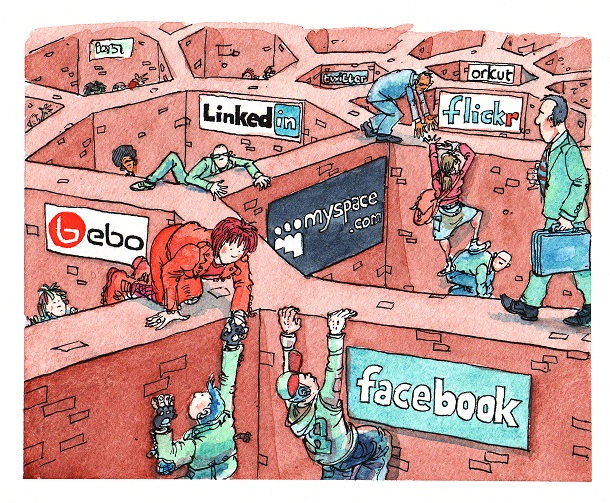
\includegraphics[width=1.0\linewidth,trim=16px 17px 12px 15px,clip]{./resources/davidsimonds.jpg}
 \caption{David Simonds illustrates social networks as walled gardens due to their (by design) lock-in effects~\cite{DavidSimonds}}
 \label{fig:DavidSimonds}
\end{figure}

%%%%%%%%%%%%%%%%%%%%%%%%%%%%
%%%  3. Media Collector  %%%
%%%%%%%%%%%%%%%%%%%%%%%%%%%%

\section{Media Collector}                                                   \label{sec:media-collector}
First, we introduce a common data format used consistently between all social networks considered.
Second, we explain the architecture for different kinds of media item extractors. Finally,
we describe the various processing steps applied to each media item collected.

%%%  3.1 Data Format  %%%
\subsection{Data Format}                                                    \label{sec:data-format}
We propose a common alignment schema for all social networks considered in Table~1 in order to be
agnostic of concrete social networks. The resulting set of metadata for a media item is detailed below:
\begin{description}
  \item[Media URL] Deep link to the media item (\url{http://farm7.staticflickr.com/6059/6290784192_567346ba6a_o.jpg}).
  \item[Type] Type of the media item (``photo'' or ``video'').
  \item[Story URL] URL of the micropost where the media item appeared (\url{http://www.flickr.com/photos/96628098@N00/6290784192/}).
  \item[Message] Text Description of the micropost in raw format (\texttt{``Laura. \#lumixg20f17, \#iswc2011, \#international\-semanticwebconference, \#bonn, \#germany''}).
  \item[Clean] Cleaned text description of the micropost where some characters are removed (\texttt{``Laura. lumixg20f17, iswc2011, internationalsemanticwebconference, bonn, germany''}).
  \item[User] URL of the micropost author (\url{http://www.flickr.com/photos/96628098@N00/}).
  \item[Published] Timestamp when the micropost was authored or the media item was uploaded (\texttt{2011\-10\-27T12:24:41Z}).
\end{description}

% Use a consistent example from one of the experiments
\autoref{lst:media} shows the sample output of a media extractor for the social network Facebook.
{\footnotesize
\begin{lstlisting}[caption={Sample output of the media extractor showing a Facebook post processed with named entity extraction and disambiguation (slightly edited for legibility).},label={lst:media}]
{
 "Facebook": [
  {
   "mediaurl": "http://video.ak.fbcdn.net/...",
   "storyurl": "https://www.facebook.com/permalink.
   php?story_fbid=231781590231029&id=1254772464",
   "message": {
    "text": "Videoed between Hamburg and Snyder.
      Thought I would share.",
    "clean": "Videoed between Hamburg and Snyder.
      Thought I would share.",
    "entities": [
     [
      {
       "name": "Hamburg",
       "relevance": 0.82274,
       "uri": "http://dbpedia.org/resource/Hamburg"
      },
      {
       "name": "Snyder",
       "relevance": 0.857,
       "uri": "http://dbpedia.org/resource/
         Snyder,_Texas"
      }
     ]
    ]
   },
   "user": "https://www.facebook.com/profile.php?
     id=1254772464",
   "type": "video",
   "timestamp": 1326371479000,
   "published": "2012-01-12T12:31:19Z"
  }
 ]
}
\end{lstlisting}}

%%%  3.2 Media Item Extractors  %%%
\subsection{Media Item Extractors}
We have developed a media collector composed of media item extractors for the seven social networks Google+, MySpace, Facebook, Twitter, Instagram, YouTube, and Flickr with additional support for the four media sharing platforms img.ly, yfrog, MobyPicture, and Twitpic. The media collector takes as input a search term that is relevant to a known event, e.g. ``costa concordia'' for the Costa Concordia Disaster. This search term gets forwarded to the search APIs of the social networks in parallel. Each social network has a 30 seconds timeout window to deliver its results. When the timeout is reached, or when all social networks have responded,
the available results are aligned according to the data format defined in \autoref{sec:data-format}. Media items are retrieved either directly or via Web scraping. For some social networks, e.g. MySpace, a combination of Web scraping and API access is required since the API does not return all necessary fields of our data format. Hence, the timestamp of when a media item is uploaded on MySpace can be obtained only via Web scraping. The complete data flow is illustrated in the architectural diagram (\autoref{fig:architecture}).
\begin{figure*}
\centering
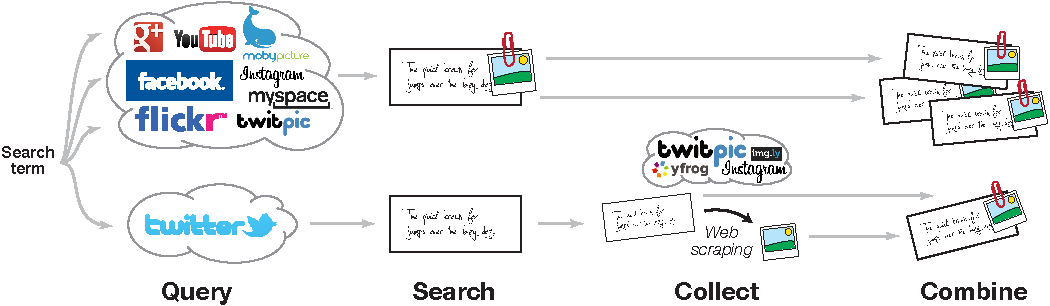
\includegraphics[width=1.0\linewidth]{./resources/architecture.pdf}
\caption{Overview of the media collector: hybrid approach for the media item extraction process using a combination of API access and Web scraping}
\label{fig:architecture}
\end{figure*}

%%%  3.3 Media Item Processing  %%%
\subsection{Media Item Processing}
As part of the processing chain, we have limited the number of returned results for each media item extractor to 10 items for videos, and 20 items for images. This explains the tendency to round numbers of results in Table~\ref{tab:number-media}, marked with $n+$.

\subsubsection{Machine Translation}
Social networking is happening at a global scale. In consequence, many microposts are authored in languages different from English. In order to still make sense out of those microposts, we apply machine translation to translate non-English microposts to English. We use the Google Translate API\footnote{\url{http://code.google.com/apis/language/translate/v2/getting_started.html}} which, if the source language parameter is left blank, tries first to detect the source language and subsequently translates the micropost to English.

\subsubsection{Part of Speech Tagging}
Our processing chain supports part of speech tagging via an open source JavaScript library called jspos\footnote{\url{http://code.google.com/p/jspos/}},
eventually based on Eric Brill's POS tagger~\cite{brill1992simple}. Part of speech tagging does not yet play an active role in the processing chain. However,
we aim for leveraging the additional data for better micropost analysis in the future.

\subsubsection{Named Entity Disambiguation}
Despite their typical relative brevity, microposts still carry a considerable amount of information. It has been shown how meaning can be added to Facebook microposts through named entity recognition and disambiguation~\cite{AddingMeaningToMicroposts}. In this paper, we generalize the approach to common microposts,
using the NERD framework~\cite{NERD}.

\subsubsection{Media Item Deduplication}
We try to evaluate the popularity of the media items shared across social networks. This task involves the deduplication of extracted media items.
For images, we use PhotoSweeper\footnote{\url{http://itunes.apple.com/us/app/photosweeper/id463362050?mt=12}}, a commercial image deduplication software and we have manually deduplicated videos. In the future, we aim to perform this task fully automatically but with this work, we have already created a baseline for specific future algorithms tailored to media item deduplication on social networks.

\paragraph{Image Deduplication}
The image duplication software we employed allows for different algorithms to be used. We have applied strict pixel-per-pixel comparison for the detection of \emph{exact} duplicates, i.e. we do \emph{not} count a resized version of an image as exact duplicate. Based on bitmap- or histogram-based similarity comparison methods, we introduce the relatively wide term of \emph{loose} duplicate. Bitmap similarity is based on comparing pixels of size-reduced bitmaps.
For our comparison, we used bitmaps of the size $128 \times 128$ pixels without smoothed edges, which corresponds to the best quality settings in the software.
Histogram similarity is based on comparing histograms of size-reduced bitmaps. This method helps finding similar images despite differences in color saturation and lighting. For both similarity comparison methods, a varying threshold was used. In our experiments, we could not make out a clear winning setting for all events. Rather, even for the same event, only a combination of both similarity comparison methods led to satisfactory results, i.e. to a set of loosely duplicate images that also a human being would have chosen. We would like to highlight, however, that all detected loosely duplicate images were detected algorithmically, which is an important fact for the objective of fully automating the deduplication process.

\paragraph{Video Deduplication}
We have deduplicated the videos in the dataset by first automatically splitting them in shots~\cite{CrowdsourcingEvent}, and then manually comparing the videos shot-wise. We considered \emph{exact} duplicates the videos that shared the same shots and same length. For \emph{loose} duplicates, we manually decided whether the videos showed loosely the same based on human judgment. We do not claim that our results are algorithmically reproducible for loosely similar video detection.

%%%%%%%%%%%%%%%%%%%%%%%%
%%%  4. Experiments  %%%
%%%%%%%%%%%%%%%%%%%%%%%%

\section{Experiments}                                                       \label{sec:experiments}
% Responsible: Thomas
For our experiments, we have taken into account several events that happened in the period of January 10 to 19, 2012, and thus were the subject of discussion on various social networks.
We have captured event-related media items and microposts, and made the data available online\footnote{Event-related media items and microposts: \url{http://webmasterapp.net/social/icmr2012/}}.
We invite the reader to browse the data and compile a personal set of loose and exact duplicate media items.
YouTube video URLs are signed with a by now expired time to live,
they can be accessed by following the \texttt{storyurl} link.

\subsection{Considered Events}
In this Subsection, we give a short overview on the context of the considered events in order to give the reader the necessary background knowledge.
% Add to each event some categorization: political, technical,…
% Add to each event the duration with start and end if possible.

\paragraph{Blackout SOPA}
The Stop Online Piracy Act (SOPA) is a bill of the United States proposed in 2011 to fight online trafficking in copyrighted intellectual property and counterfeit goods.
On January 18, the English Wikipedia, Reddit, and several other Internet companies coordinated a service blackout to protest SOPA and its sister bill, the Protect IP Act.
Other companies, including Google, posted links and images in an effort to raise awareness.
% \footnote{Blackout SOPA: \url{http://sopablackout.org/learnmore/}}

\paragraph{Assad Speech}
On January 10, 2012, Syrian President Bashar al-Assad delivered a lengthy televised talk strongly defending his government's actions and motivations, despite world pressure on his embattled government for its 10-month crackdown on protesters.
% \footnote{Assad Speech: \url{http://www.cnn.com/2012/01/10/world/meast/syria-unrest/}}

\paragraph{Christian Wulff Case}
Since December 2011, German President Christian Wulff faces controversy over discrepancies in statements about a loan while governor of Lower Saxony.
When the affair settled down, it was revealed that he had applied pressure on Springer Press to delay revelations on the issue until he was back from a visit abroad.
When Wulff found out that a tabloid was going to break the story, he left a message on the voice mail of the editor-in-chief in which he threatened to take legal action.
% \footnote{Christian Wulff Case: \url{http://www.spiegel.de/international/germany/0,1518,804631,00.html}}

\paragraph{Dixville Notch}
Dixville Notch is an unincorporated village in Dixville township of Coos County, New Hampshire, USA, best known in connection with its longstanding middle-of-the-night vote in the U.S. presidential election.
In a tradition that started in the 1960 election, all the eligible voters in Dixville Notch gather at midnight in the ballroom of The Balsams.
This year, on January 10, 2012, the voters cast their ballots and the polls officially closed one minute later.
% \footnote{Dixville Notch: \url{http://www.washingtonpost.com/2012/01/09/gIQANslKnP_story.html}}

\paragraph{Free Mobile Launch}
Free Mobile is a French mobile broadband company, part of the Iliad group.
On January 10, 2012, a long-awaited mobile phone package for \EUR{19.99} with calls included to 40 countries, texts, multimedia messages and Internet was announced by the Iliad group's Chief Strategy Officer, Xavier Niel.
% \footnote{Free Mobile Launch: \url{http://www.nytimes.com/2012/01/11/technology/iliad-takes-aim-at-top-mobile-operators-in-france.html}}

\paragraph{Costa Concordia Disaster} \label{sec:concordia}
The Costa Concordia is an Italian cruise ship that hit a reef and partially sank on January 13, 2012 off the Italian coast.
The vessel ran aground at Isola del Giglio, Tuscany, resulting in the evacuation of 4,211 people on board.
% \footnote{Coosta Concordia Disaster: \url{http://www.costacruise.com/B2C/USA/Info/concordia_statement.htm}}

\paragraph{CES Las Vegas}
The International Consumer Electronics Show (CES) is a major technology-related trade show held each January in the Las Vegas Convention Center.
Not open to the public, the Consumer Electronics Association-sponsored show typically hosts previews of products and new product announcements.
% \footnote{CES Las Vegas: \url{http://www.cesweb.org/aboutcea.asp}}

\paragraph{Cut the Rope Launch}
% Sub-event of CES Las Vegas
On January 10, 2012 during Microsoft's keynote at CES, the HTML5 version of the popular mobile game \textit{Cut the Rope} was announced.
% \footnote{Cut the Rope Launch: \url{http://ces.cnet.com/8301-33377_1-57356403/}}

\paragraph{Ubuntu TV Launch}
% Sub-event of CES Las Vegas
Ubuntu TV by Canonical, based on the user interface Unity, is a variant of the Ubuntu operating system, designed to be a Linux distribution specially adapted for embedded systems in televisions. It was announced by Canonical on January 10, 2012, at CES.
% \footnote{Ubuntu TV: \url{http://www.theverge.com/2012/1/9/2695387/ubuntu-tv-video-hands-on}}

\subsection{Dataset} \label{subsec:dataset}
Our data set contained 448 images with an average file size of $\sim$0.7MB and 143 videos.
During the examination of our dataset, we observed that the process of image deduplication is by no means a solved issue.
Content-based image retrieval (CBIR) uses features like color, texture, and shape to search images from large-scale databases.
The same technique, however, can also be used for the deduplication of photographs~\cite{Pattabhi:RAICS11}.
We used a CBIR-based image duplication detection software\footnote{PhotoSweeper: \url{http://itunes.apple.com/us/app/photosweeper/id463362050?mt=12}} that allows for manual algorithm and threshold selection to detect duplicates in the dataset.
For each considered event, we manually selected the best settings to limit the number of duplicate misses and false positives.
The main problem with the dataset is its diversity.
It ranges from entirely sharp screenshots in all sorts of formats (e.g., screenshots of the Google homepage for the Blackout SOPA event), to blurry cell phone images in standard photo formats (e.g., photos of the stage for the Free Mobile Launch event).
A common performance tweak to speed up the duplication detection process is to shrink images to quadratic bitmaps.
In the context of our dataset, however, this approach is counterproductive, as a screenshot of a rectangular IAB $728 \times 90$ ``leaderboard'' banner is treated the same as a standard 3.1 megapixels ($2048 \times 1536$) cell phone photo.
In practice, shrinking a wide rectangular banner to a square led to many incorrect results, requiring manual deduplication with the Blackout SOPA event.

\begin{table*}[htbp]
  \centering{
  \small{
  \begin{tabular}{|c|c|c|c|c|c|c|c|c|c|c|c|c|c|c|c|c|c|c|}
    \hline
    \multicolumn{1}{|c|}{\textbf{Social}} & \multicolumn{2}{c|}{\textbf{Assad}} & \multicolumn{2}{c|}{\textbf{CES}} &
    \multicolumn{2}{c|}{\textbf{Concordia}} & \multicolumn{2}{c|}{\textbf{Dixville}} & \multicolumn{2}{c|}{\textbf{Free}} &
    \multicolumn{2}{c|}{\textbf{Ropes}} & \multicolumn{2}{c|}{\textbf{SOPA}} & \multicolumn{2}{c|}{\textbf{Ubuntu}} &
    \multicolumn{2}{c|}{\textbf{Wulff}} \\
    \cline{2-19}
    \multicolumn{1}{|c|}{\textbf{Network}} & \textbf{I} & \textbf{V} & \textbf{I} & \textbf{V} & \textbf{I} & \textbf{V} &
    \textbf{I} & \textbf{V} & \textbf{I} & \textbf{V} & \textbf{I} & \textbf{V} & \textbf{I} & \textbf{V} & \textbf{I} &
    \textbf{V} & \textbf{I} & \textbf{V} \\
    \hline
    \textbf{Google+} & 3 & 2 & 5 & 3 & 15 & 1 & 4 & 1 & 6 & 0 & 5 & 1 & 5 & 0 & 6 & 1 & 7 & 0\\
    \textbf{MySpace} & 0 & 0 & 0 & 0 & 10+ & 0 & 9 & 0 & 1 & 0 & 6 & 0 & 0 & 0 & 0 & 0 & 8 & 0\\
    \textbf{Facebook} & 0 & 0 & 0 & 1 & 0 & 1 & 0 & 0 & 0 & 0 & 0 & 0 & 0 & 2 & 0 & 0 & 0 & 0\\
    \textbf{Twitter} & 2 & 0 & 2 & 0 & 3 & 0 & 3 & 0 & 2 & 0 & 4 & 0 & 5 & 0 & 0 & 0 & 2 & 0\\
    \textbf{Instagram} & 0 & 0 & 20+ & 0 & 20+ & 0 & 0 & 0 & 20+ & 0 & 20+ & 0 & 20+ & 0 & 0 & 0 & 2 & 0\\
    \textbf{YouTube} & 0 & 10+ & 0 & 10+ & 0 & 10+ & 0 & 3 & 0 & 10+ & 0 & 10+ & 0 & 10+ & 0 & 10+ & 0 & 10+\\
    \textbf{Flickr} & 10+ & 0 & 10+ & 6 & 10+ & 10+ & 10+ & 10+ & 10+ & 0 & 10+ & 10+ & 10+ & 0 & 10+ & 9 & 10+ & 2\\
    \textbf{MobyPicture} & 0 & 0 & 1 & 0 & 4 & 0 & 0 & 0 & 2 & 0 & 20+ & 0 & 1 & 0 & 2 & 0 & 3 & 0\\
    \textbf{Twitpic} & 0 & 0 & 20+ & 0 & 18 & 0 & 1 & 0 & 20+ & 0 & 20+ & 0 & 19 & 0 & 2 & 0 & 20+ & 0\\
    \hline
    \textbf{Total} & 15 & 12 & 58 & 20 & 80 & 22 & 27 & 14 & 61 & 10 & 85 & 21 & 60 & 12 & 20 & 20 & 52 & 12\\
    \hline
  \end{tabular}
  }
  \label{tab:number-media}
  \caption{Number of images and videos collected for the 9 events (resp. \textbf{Assad Speech}, \textbf{CES Las Vegas}, \textbf{Costa Concordia Disaster}, \textbf{Dixville Notch}, \textbf{Free Mobile Launch}, \textbf{Cut the Rope Launch}, \textbf{Blackout SOPA}, \textbf{Ubuntu TV Launch} and \textbf{Christian Wulff Case}) grouped by social networks}
  }
\end{table*}

\begin{table*}[htbp]
  \begin{tabular}{ | c | c | c | }
    \hline
    \textbf{Event} & \textbf{Exact Duplicate Images} & \textbf{Loose Duplicate Images}\\
    \hline
    Assad Speech & 0 images in 0 sequences & 2 images in 1 sequence\\
    Blackout SOPA & 0 images in 0 sequences & 14 images in 4 sequences\\
    CES Las Vegas & 0 images in 0 sequences & 9 images in 3 sequences\\
    Christian Wulff Case & 4 images in 2 sequences & 0 images in 0 sequences\\
    Costa Concordia & 0 images in 0 sequences & 6 images in 3 sequences\\
    Cut the Rope Launch & 2 images in 1 sequence & 15 images in 5 sequences\\
    Dixville Notch & 2 images in 1 sequence & 2 images in 1 sequence\\
    Free Mobile Launch & 2 images in 1 sequence & 16 images in 7 sequences\\
    Ubuntu TV Launch & 0 images in 0 sequences & 5 images in 1 sequence\\
    \hline
  \end{tabular}
  \label{tab:duplicateimages}
  \caption{Exact and loose duplicate images per event.}
\end{table*}

\begin{table*}[htbp]
  \begin{tabular}{ | c | c | c | }
    \hline
    \textbf{Event} & \textbf{Exact Duplicate Videos} & \textbf{Loose Duplicate Videos}\\
    \hline
    Assad Speech\footnote{3 videos were no longer available due to account termination by the users (two cases) and video takedown by the user (one case).}\todo{Footnote not shown. Needs manual fix?} & 0 videos in 0 sequences & 2 videos in 1 sequence\\
    Blackout SOPA & 2 videos in 1 sequence & 0 videos in 0 sequences\\
    CES Las Vegas & 0 videos in 0 sequences & 2 videos in 1 sequence\\
    Christian Wulff Case & 0 videos in 0 sequences & 0 videos in 0 sequences\\
    Costa Concordia & 0 videos in 0 sequences & 0 videos in 0 sequences\\
    Cut the Rope Launch & 0 videos in 0 sequences & 14 videos in 3 sequences\footnote{6 videos in 2 sequences were false positives.}\todo{Footnote not shown. Needs manual fix?}\\
    Dixville Notch & 2 videos in 1 sequence & 0 videos in 0 sequences\footnote{1 video was no longer available due to video takedown by the user. 11 videos were false positives.}\todo{Footnote not shown. Needs manual fix?}\\
    Free Mobile Launch & 0 videos in 0 sequences & 0 videos in 0 sequences\footnote{5 videos were false positives.}\todo{Footnote not shown. Needs manual fix?}\\
    Ubuntu TV Launch & 4 videos in 1 sequence & 9 videos in 4 sequences\footnote{8 videos in 3 sequences were false positives.}\todo{Footnote not shown. Needs manual fix?}\\
    \hline
  \end{tabular}
  \label{tab:duplicatevideos}
  \caption{Exact and loose duplicate videos per event.}
\end{table*}

\begin{figure*}
\begin{tabular}{p{\textwidth}}
\eventtitle{Blackout SOPA}
\begin{thumbsequence}
		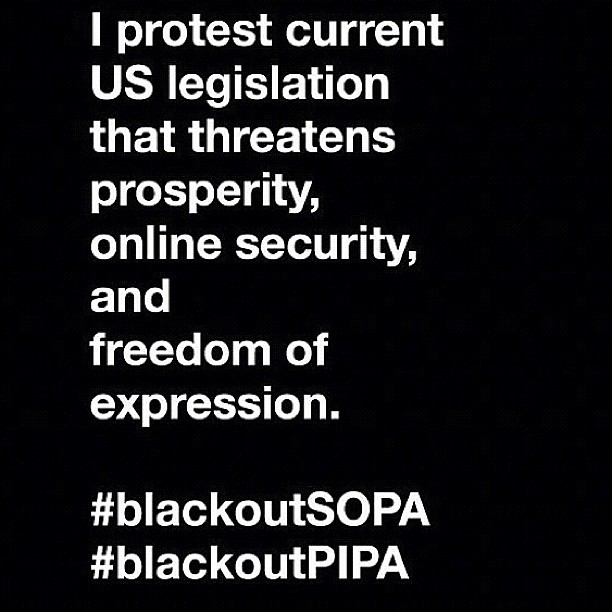
\includegraphics[height=\thumbheight]{resources/sopa/looseduplicate1.jpg}
		
\includegraphics[height=\thumbheight]{resources/sopa/looseduplicate2.jpg}
		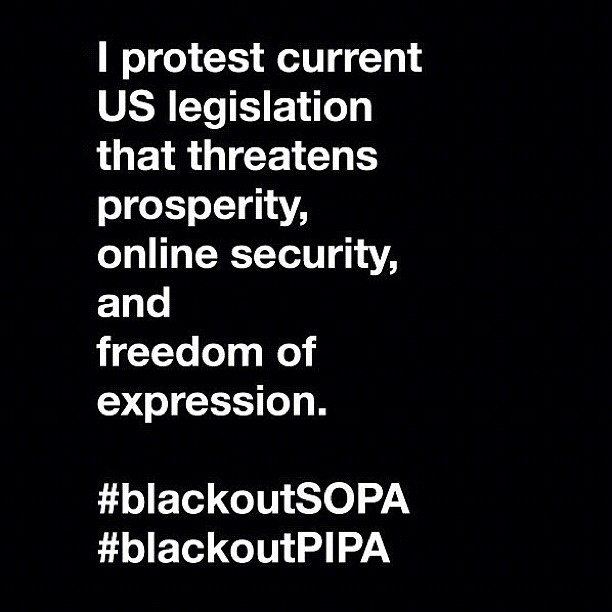
\includegraphics[height=\thumbheight]{resources/sopa/looseduplicate3.jpg}
		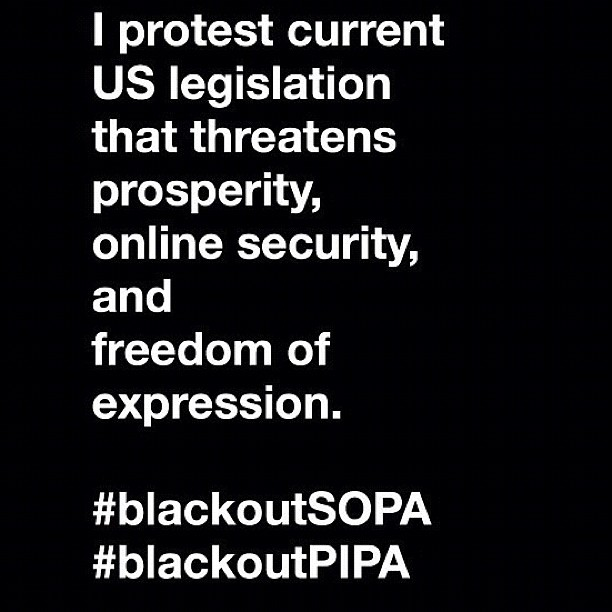
\includegraphics[height=\thumbheight]{resources/sopa/looseduplicate4.jpg}
		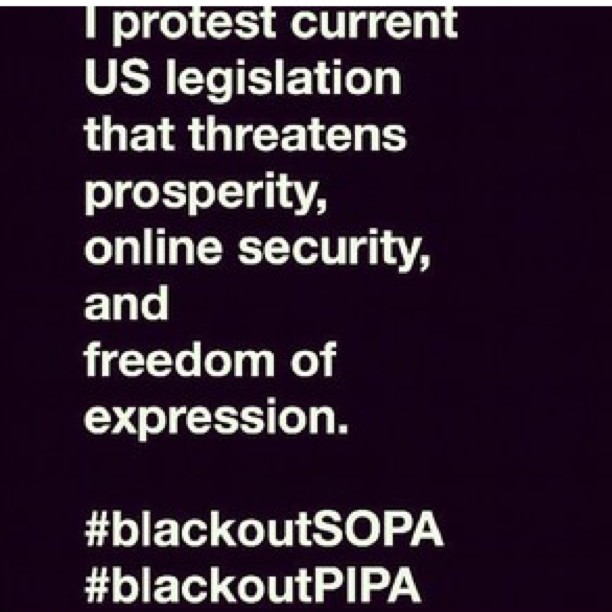
\includegraphics[height=\thumbheight]{resources/sopa/looseduplicate5.jpg}
		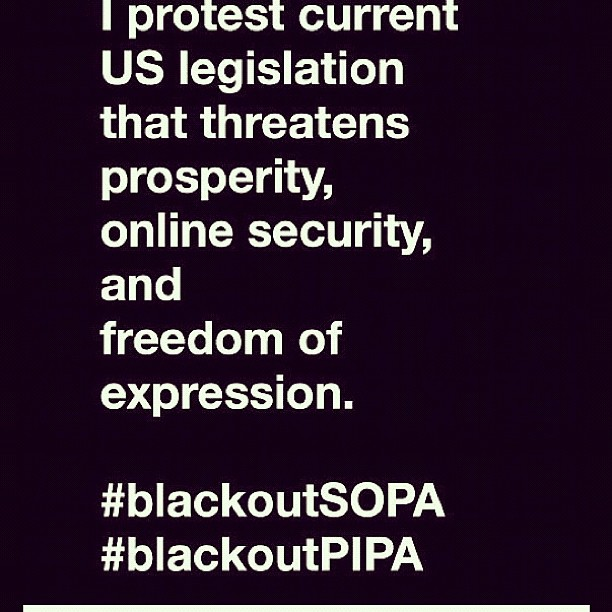
\includegraphics[height=\thumbheight]{resources/sopa/looseduplicate6.jpg}
	\end{thumbsequence}
	\begin{thumbsequence}
		
\includegraphics[height=\thumbheight]{resources/sopa/looseduplicate7.png}
		
\includegraphics[height=\thumbheight]{resources/sopa/looseduplicate8.jpg}
	\end{thumbsequence}
	\newstrip
	\begin{thumbsequence}
		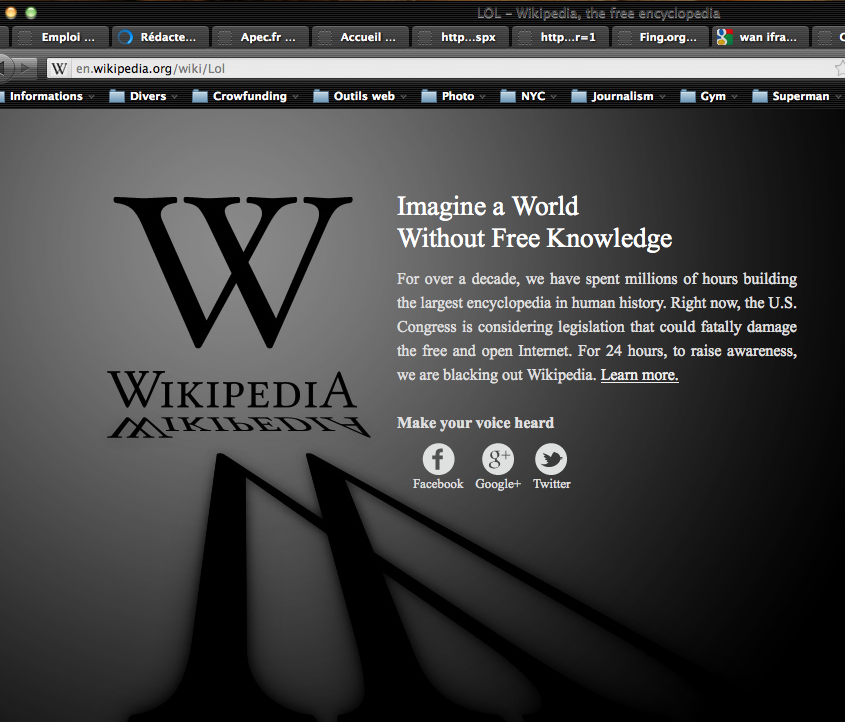
\includegraphics[height=\thumbheight]{resources/sopa/looseduplicate9.png}
		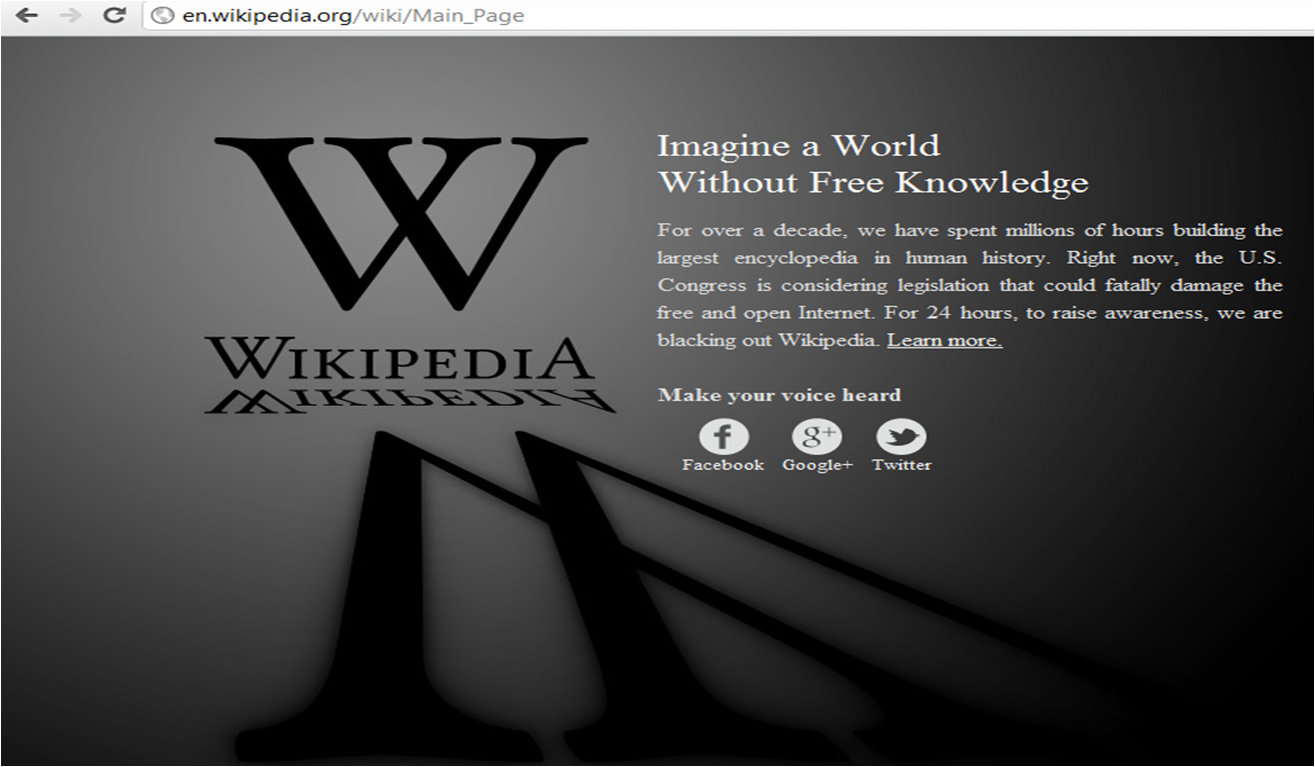
\includegraphics[height=\thumbheight]{resources/sopa/looseduplicate10.png}
		
\includegraphics[height=\thumbheight]{resources/sopa/looseduplicate11.jpg}
		
\includegraphics[height=\thumbheight]{resources/sopa/looseduplicate12.jpg}
	\end{thumbsequence}
	\begin{thumbsequence}
		\setlength\fboxsep{0pt}
		\setlength\fboxrule{0.1mm}
		\fbox{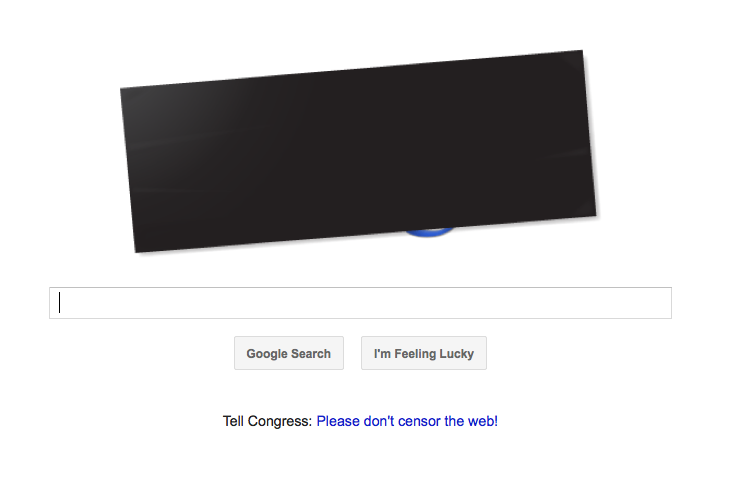
\includegraphics[height=\thumbheight]{resources/sopa/looseduplicate13.png}}
		\fbox{
\includegraphics[height=\thumbheight]{resources/sopa/looseduplicate14.jpg}}
\end{thumbsequence}
\end{tabular}

\vspace{.5em}
	
\begin{tabular}{p{\textwidth}}
\eventtitle{Christian Wulff Case}
	\begin{thumbsequence}
		\doublebox{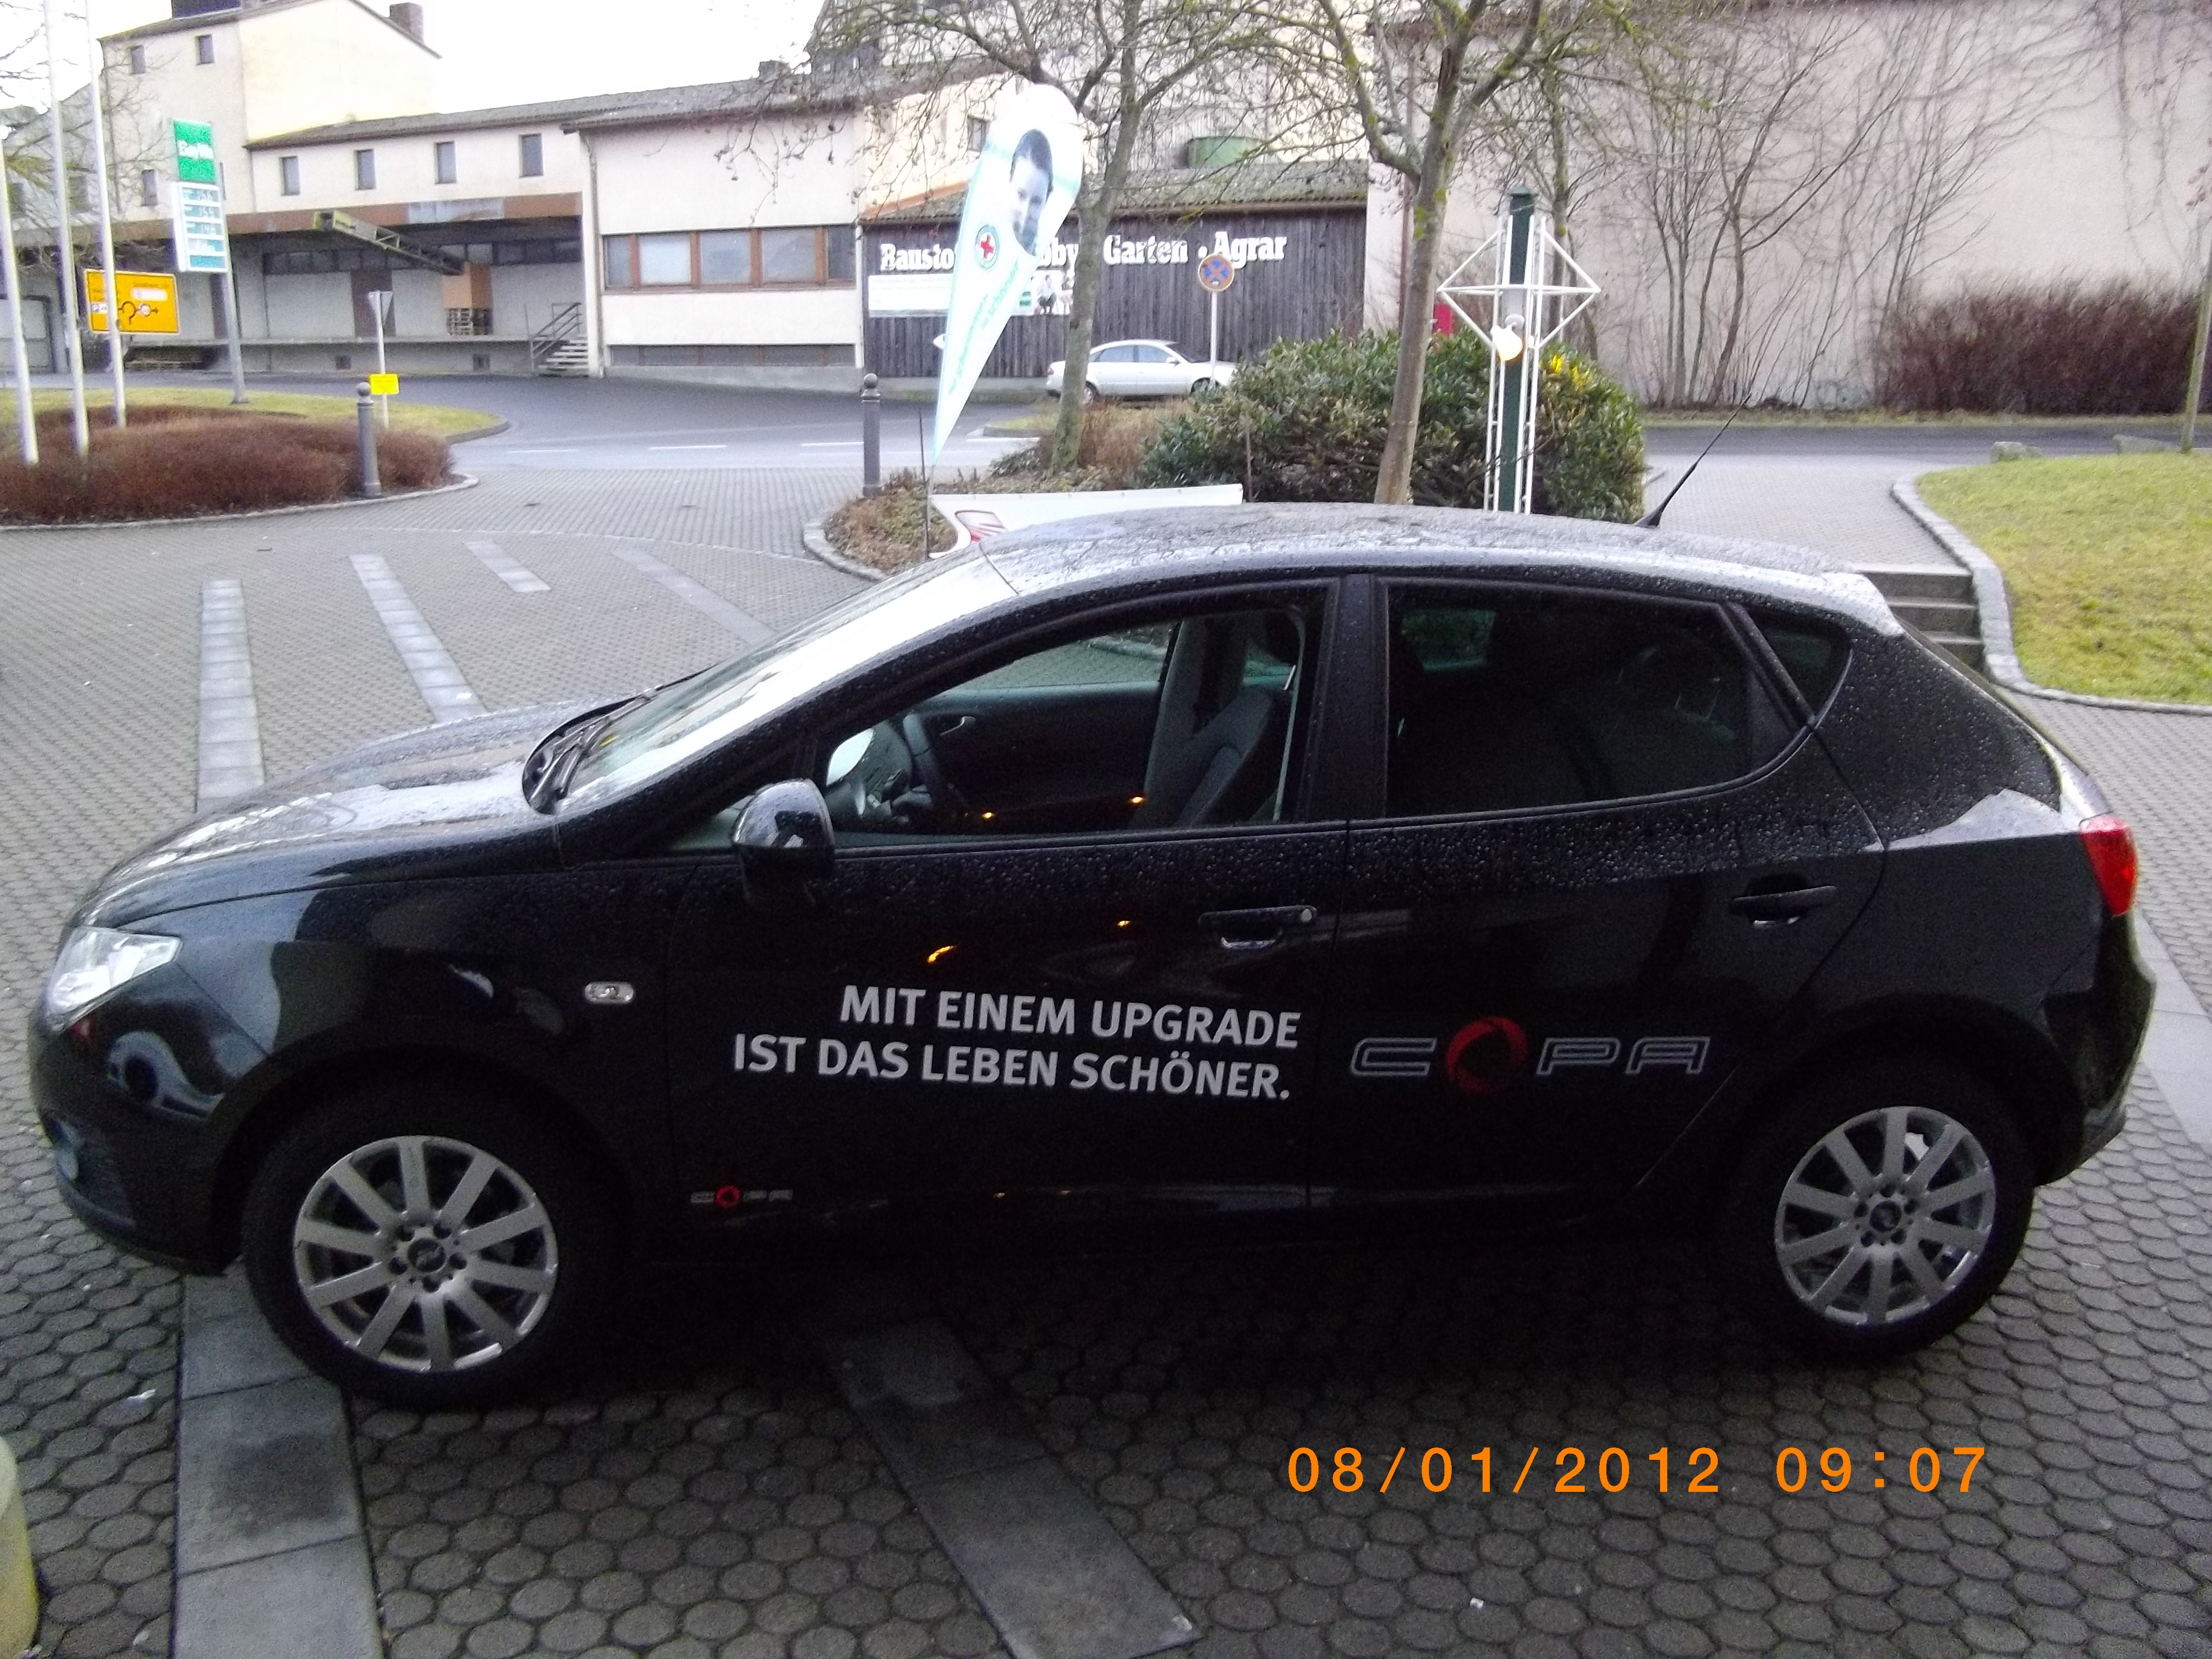
\includegraphics[height=\thumbheight]{resources/wulff/exactduplicate1.jpg}}
		\doublebox{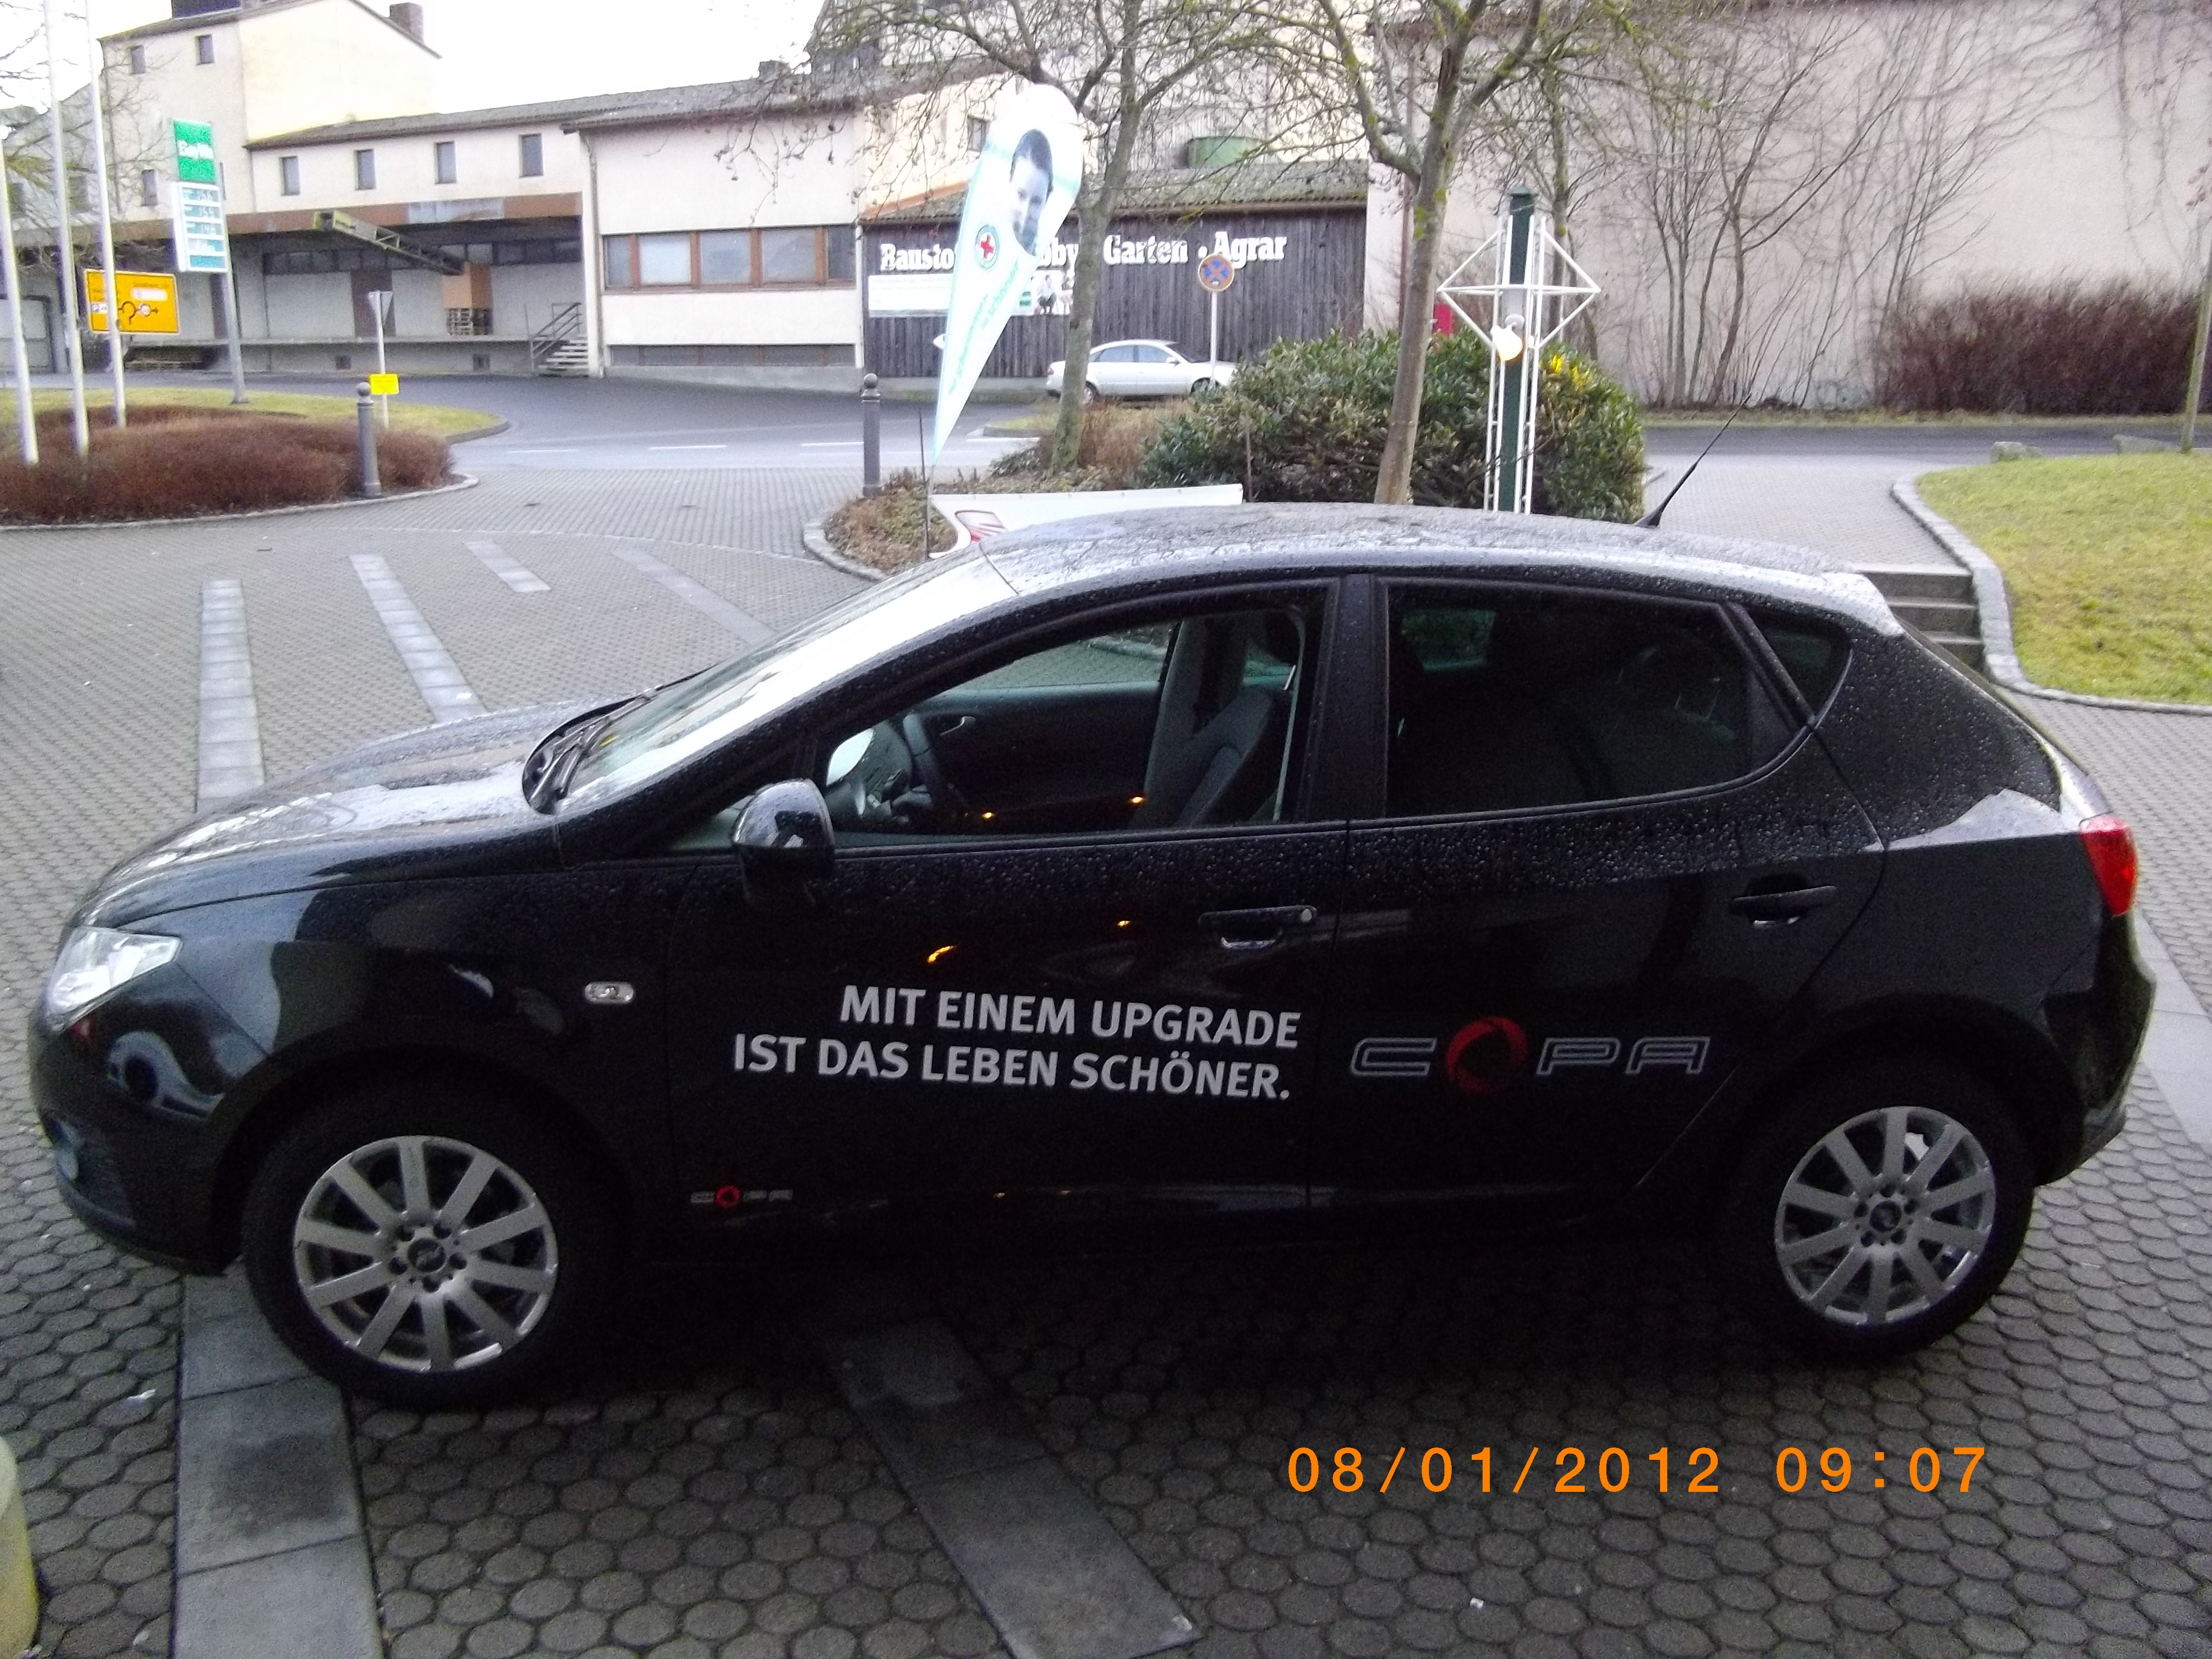
\includegraphics[height=\thumbheight]{resources/wulff/exactduplicate2.jpg}}
	\end{thumbsequence}
	\begin{thumbsequence}
		\doublebox{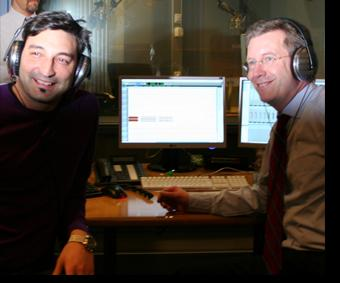
\includegraphics[height=\thumbheight]{resources/wulff/exactduplicate3.jpg}}
		\doublebox{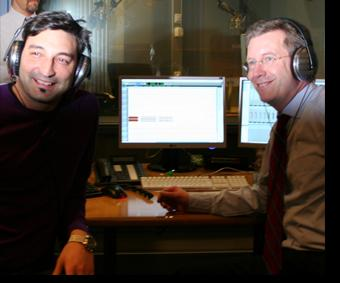
\includegraphics[height=\thumbheight]{resources/wulff/exactduplicate4.jpg}}
	\end{thumbsequence}
\end{tabular}

\vspace{.5em}

\begin{tabular}{p{.5\textwidth}p{.5\textwidth}}
\eventtitle{Dixville Notch}
	\begin{thumbsequence}
		\doublebox{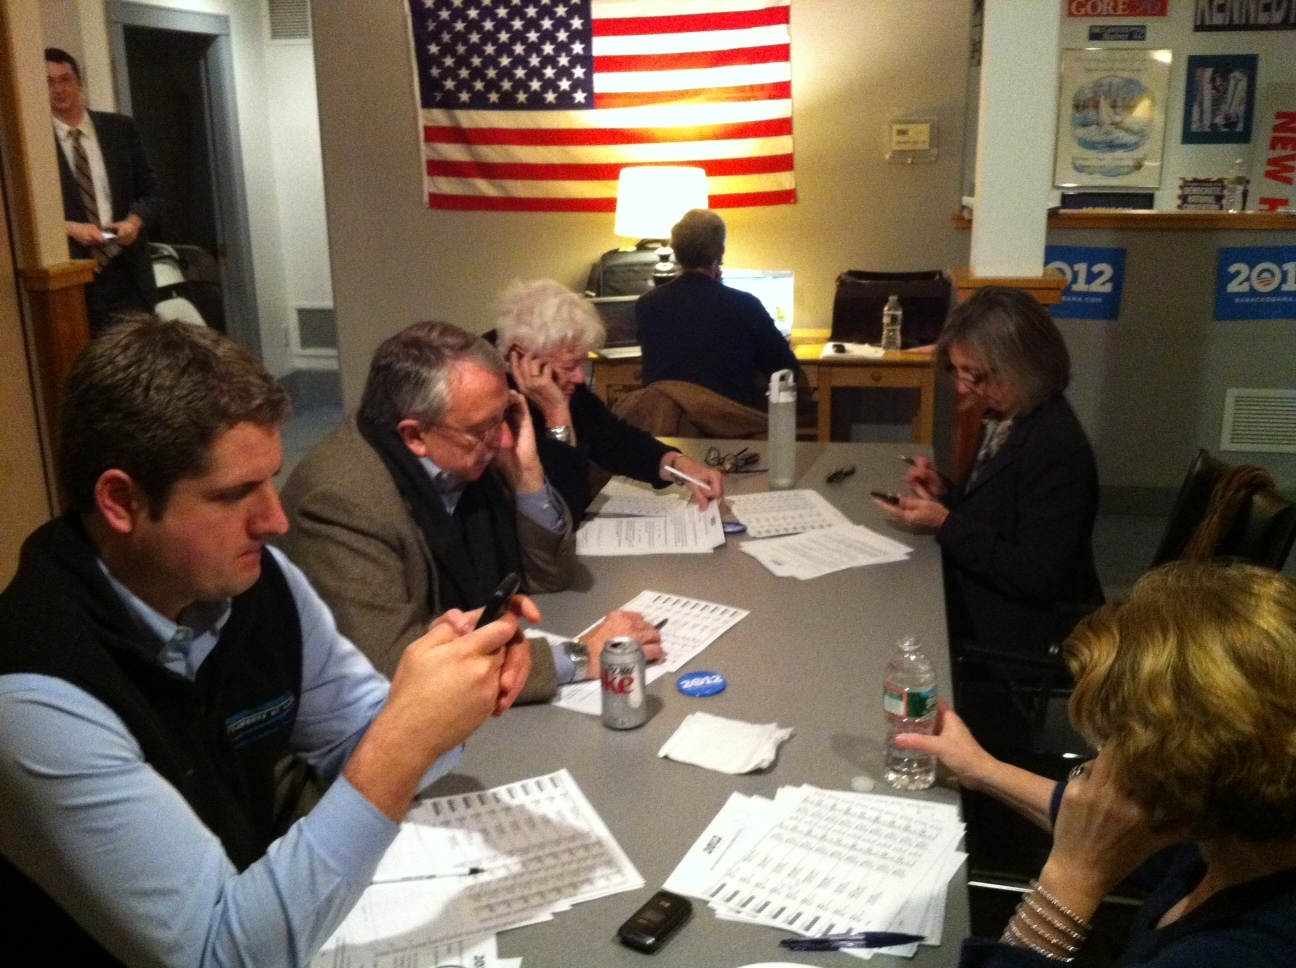
\includegraphics[height=\thumbheight]{resources/dixville/exactduplicate1.jpg}}
		\doublebox{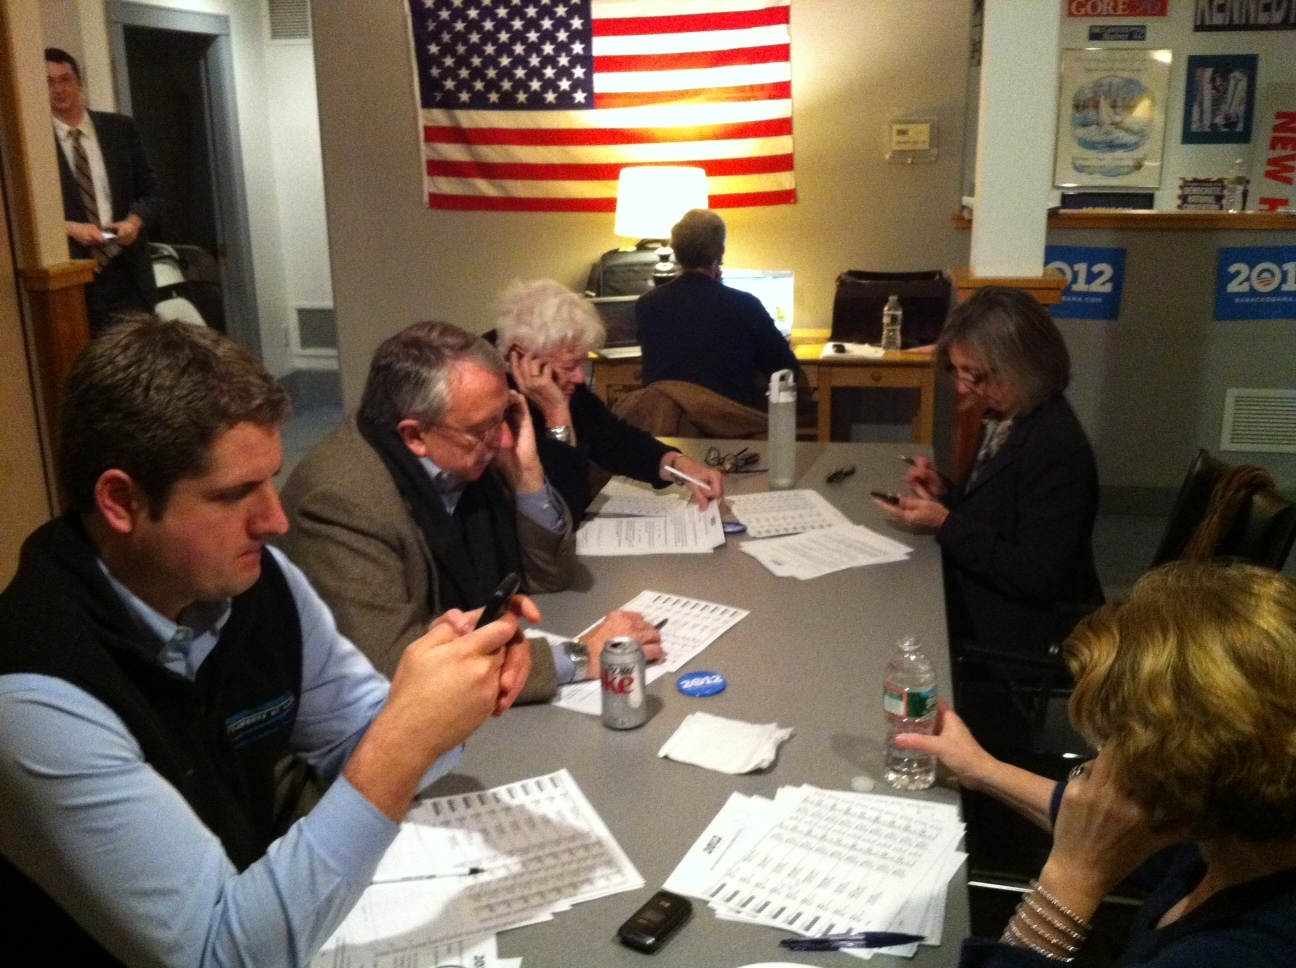
\includegraphics[height=\thumbheight]{resources/dixville/exactduplicate2.jpg}}
	\end{thumbsequence}
	\begin{thumbsequence}
		\includegraphics[height=\thumbheight]{resources/dixville/looseduplicate1.jpg}
		
\includegraphics[height=\thumbheight]{resources/dixville/looseduplicate2.jpg}
	\end{thumbsequence}
	&
\vspace{-3pt}
\eventtitle{Assad Speech}
	\begin{thumbsequence}
		\includegraphics[height=\thumbheight]{resources/assad/looseduplicate1.jpg}
		
\includegraphics[height=\thumbheight]{resources/assad/looseduplicate2.jpg}
	\end{thumbsequence}
\end{tabular}

\vspace{.5em}

\begin{tabular}{p{\textwidth}}
\eventtitle{Free Mobile Launch}
	\begin{thumbsequence}
		\doublebox{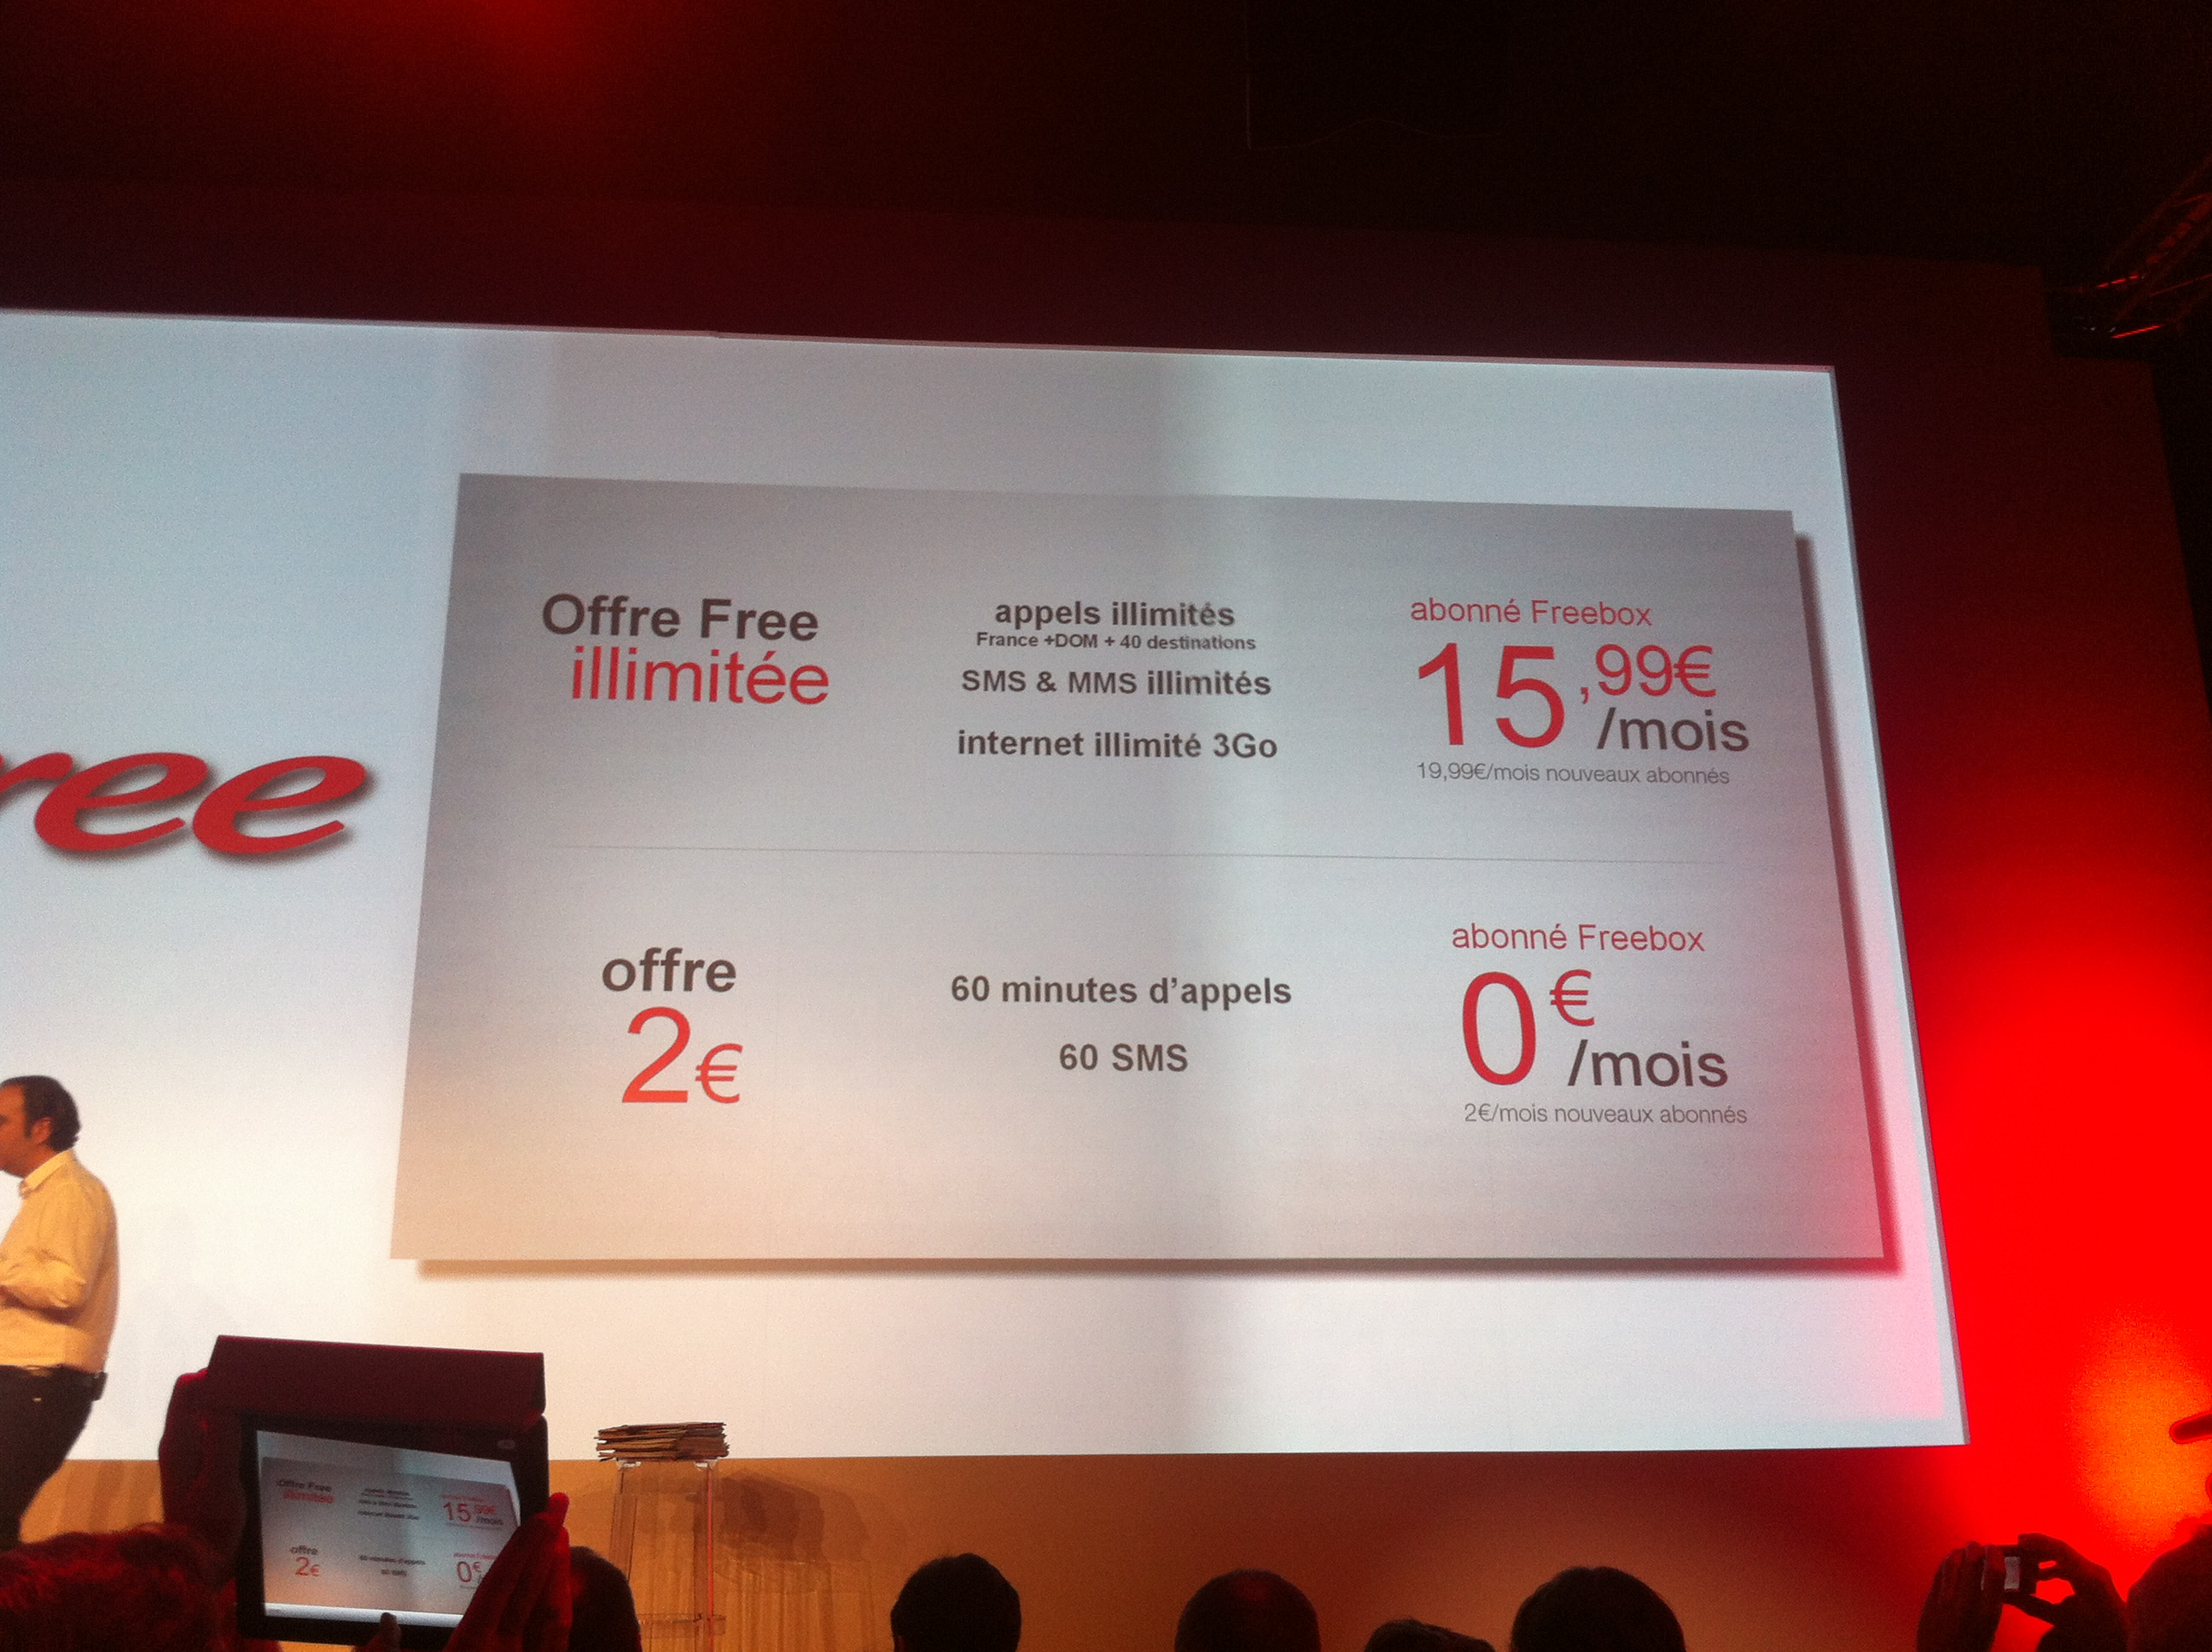
\includegraphics[height=\thumbheight]{resources/free/exactduplicate1.jpg}}
		\doublebox{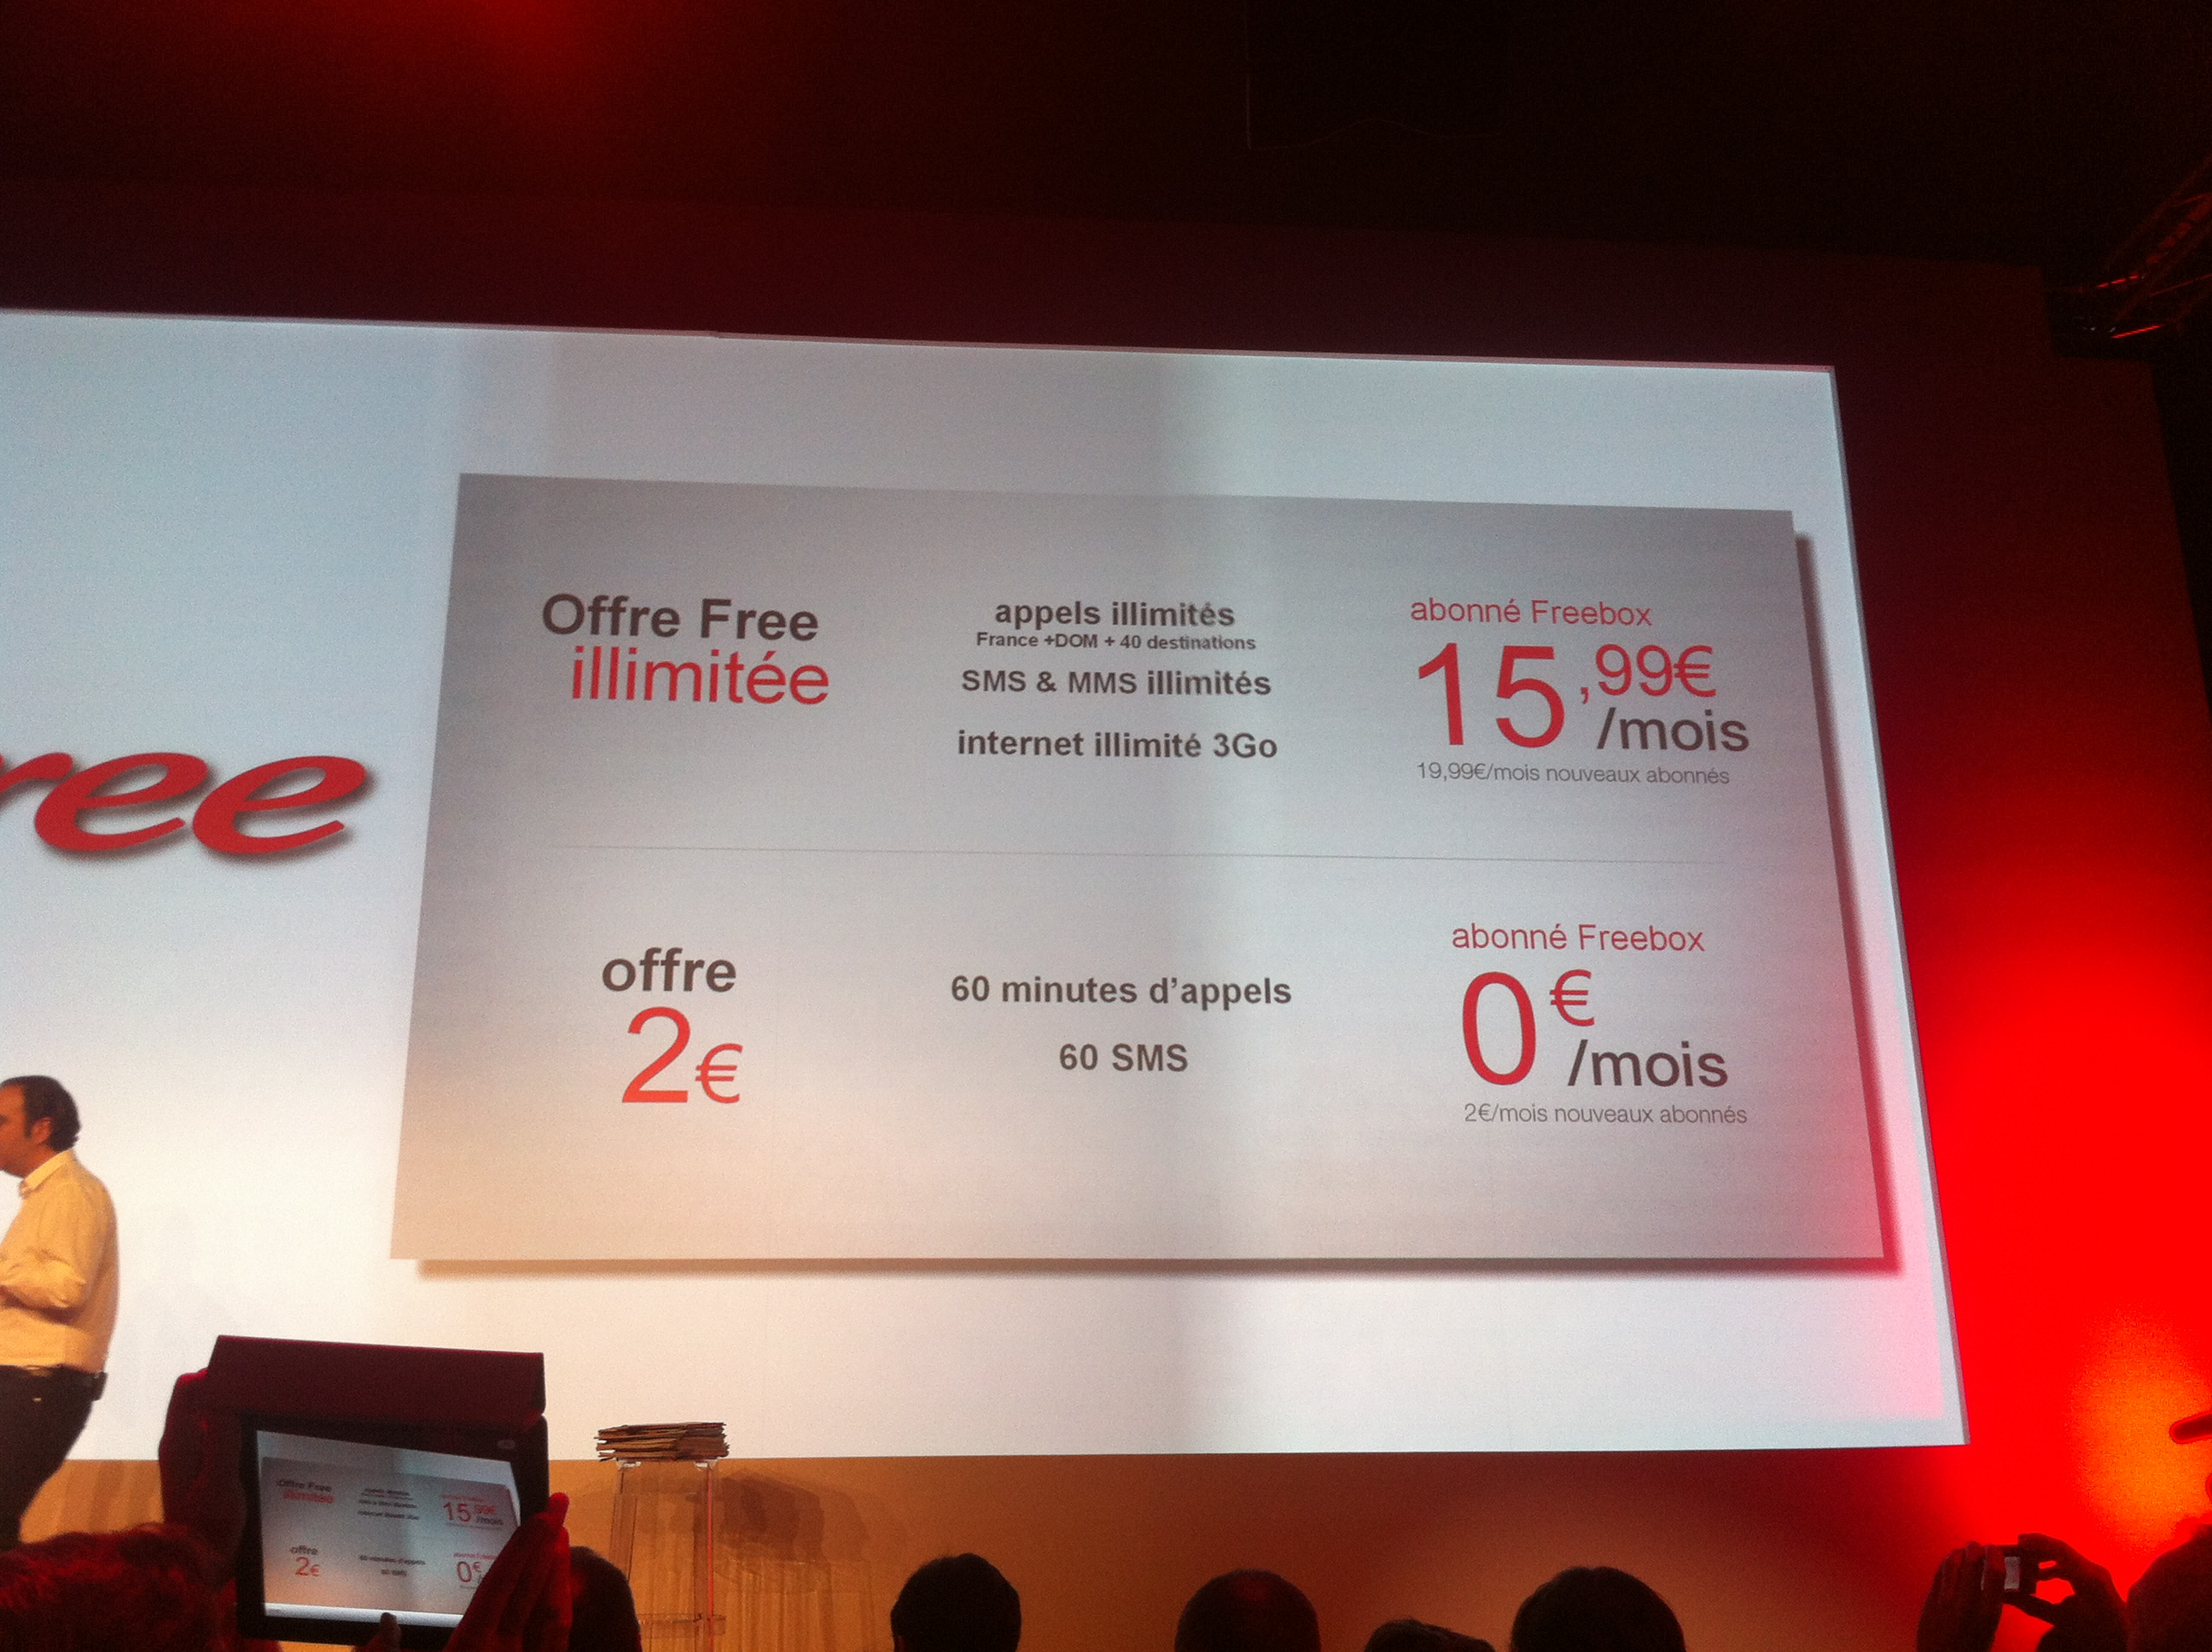
\includegraphics[height=\thumbheight]{resources/free/exactduplicate2.jpg}}
	\end{thumbsequence}
	\begin{thumbsequence}
		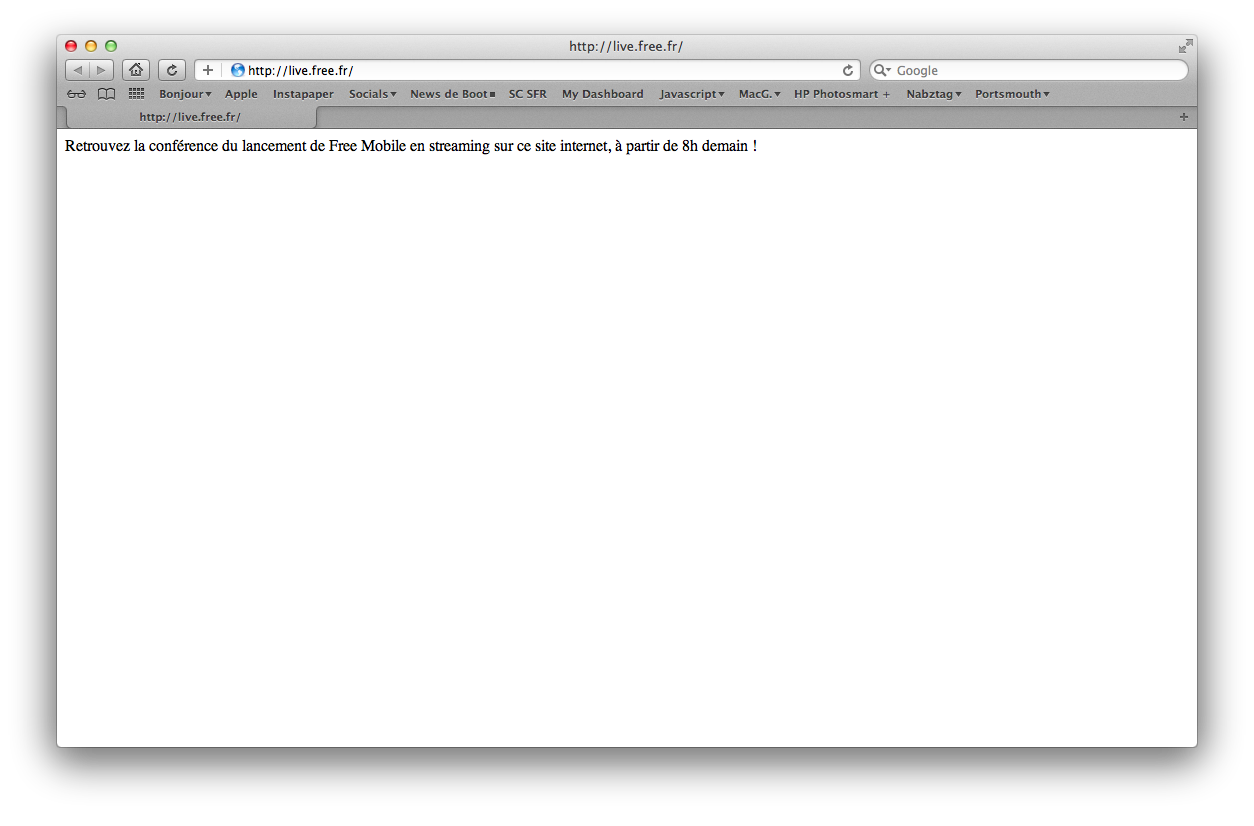
\includegraphics[height=\thumbheight]{resources/free/looseduplicate1.png}
		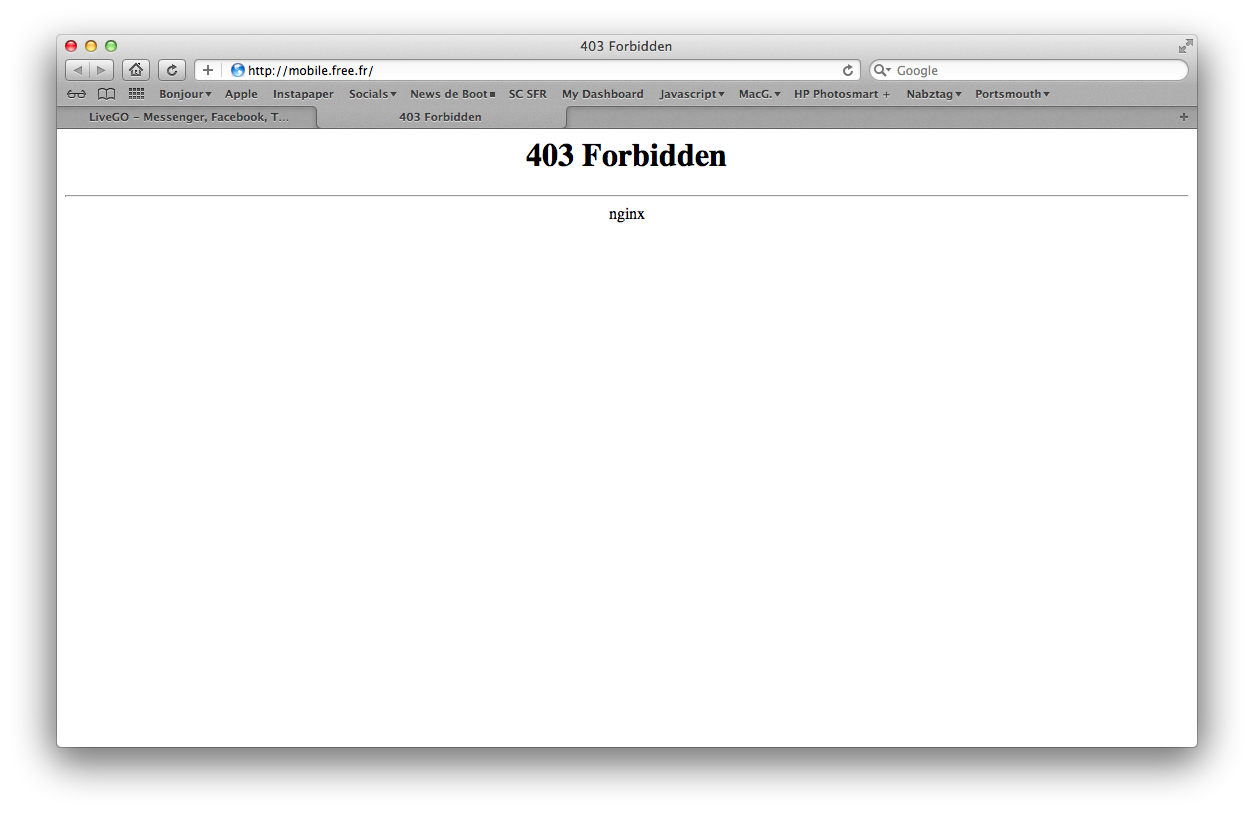
\includegraphics[height=\thumbheight]{resources/free/looseduplicate2.png}
	\end{thumbsequence}
	\begin{thumbsequence}
		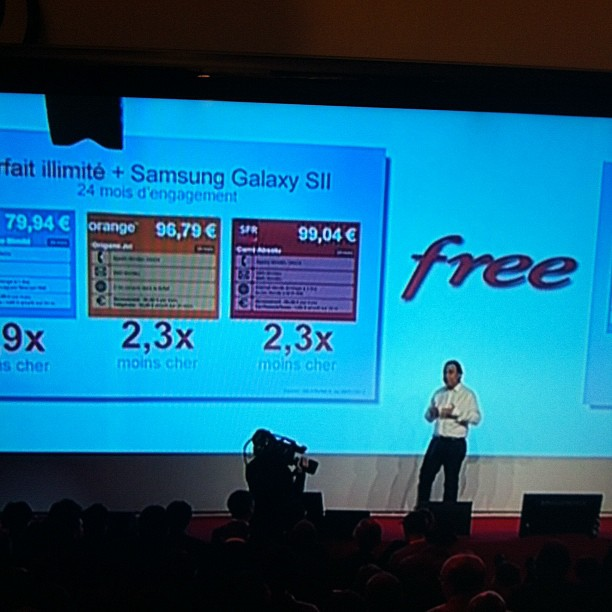
\includegraphics[height=\thumbheight]{resources/free/looseduplicate7.jpg}
		
\includegraphics[height=\thumbheight]{resources/free/looseduplicate8.jpg}
	\end{thumbsequence}
	\\[4pt]
	\begin{thumbsequence}
		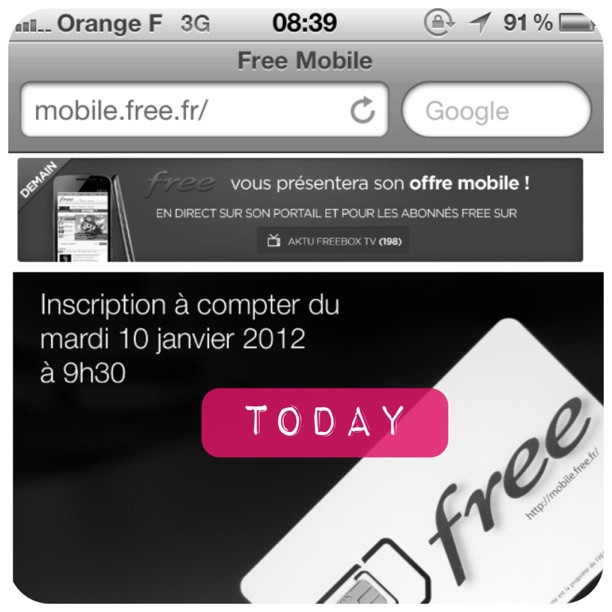
\includegraphics[height=\thumbheight]{resources/free/looseduplicate15.jpg}
		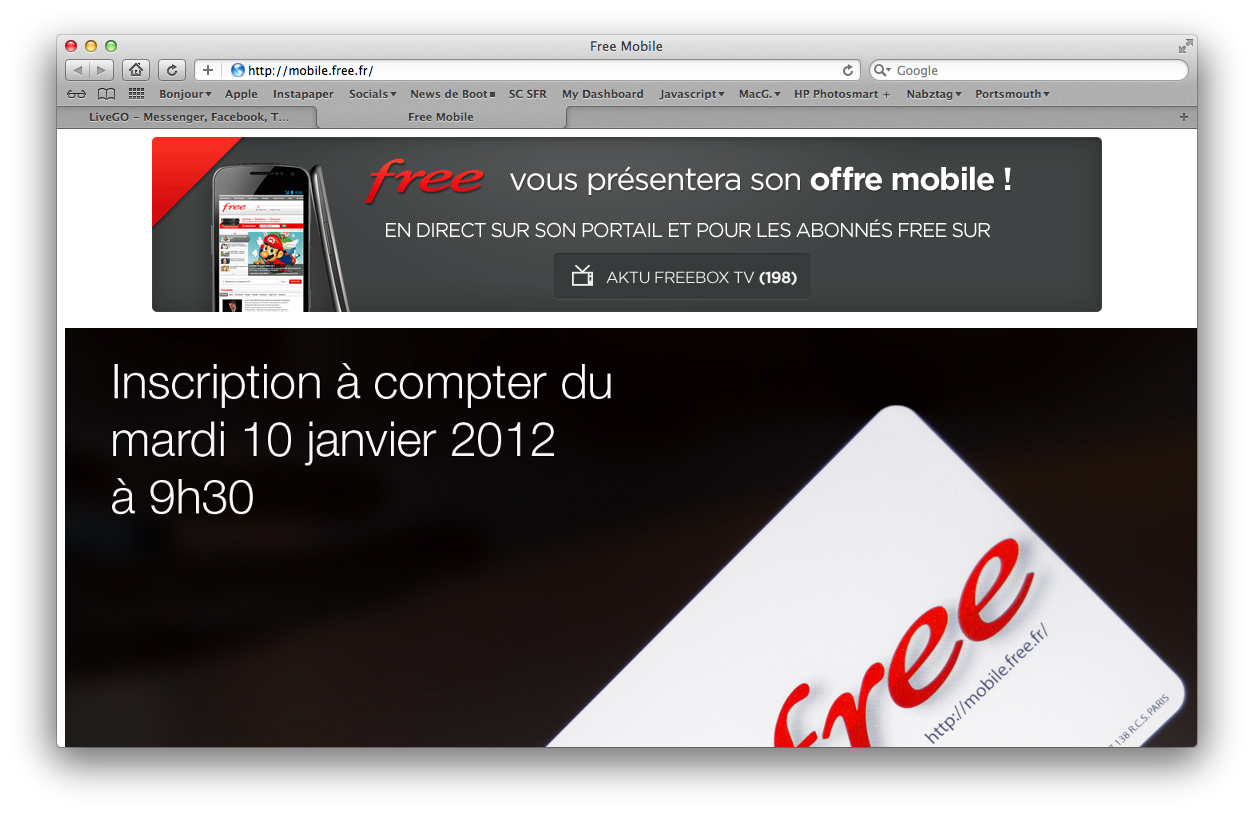
\includegraphics[height=\thumbheight]{resources/free/looseduplicate16.png}
	\end{thumbsequence}
	\begin{thumbsequence}
		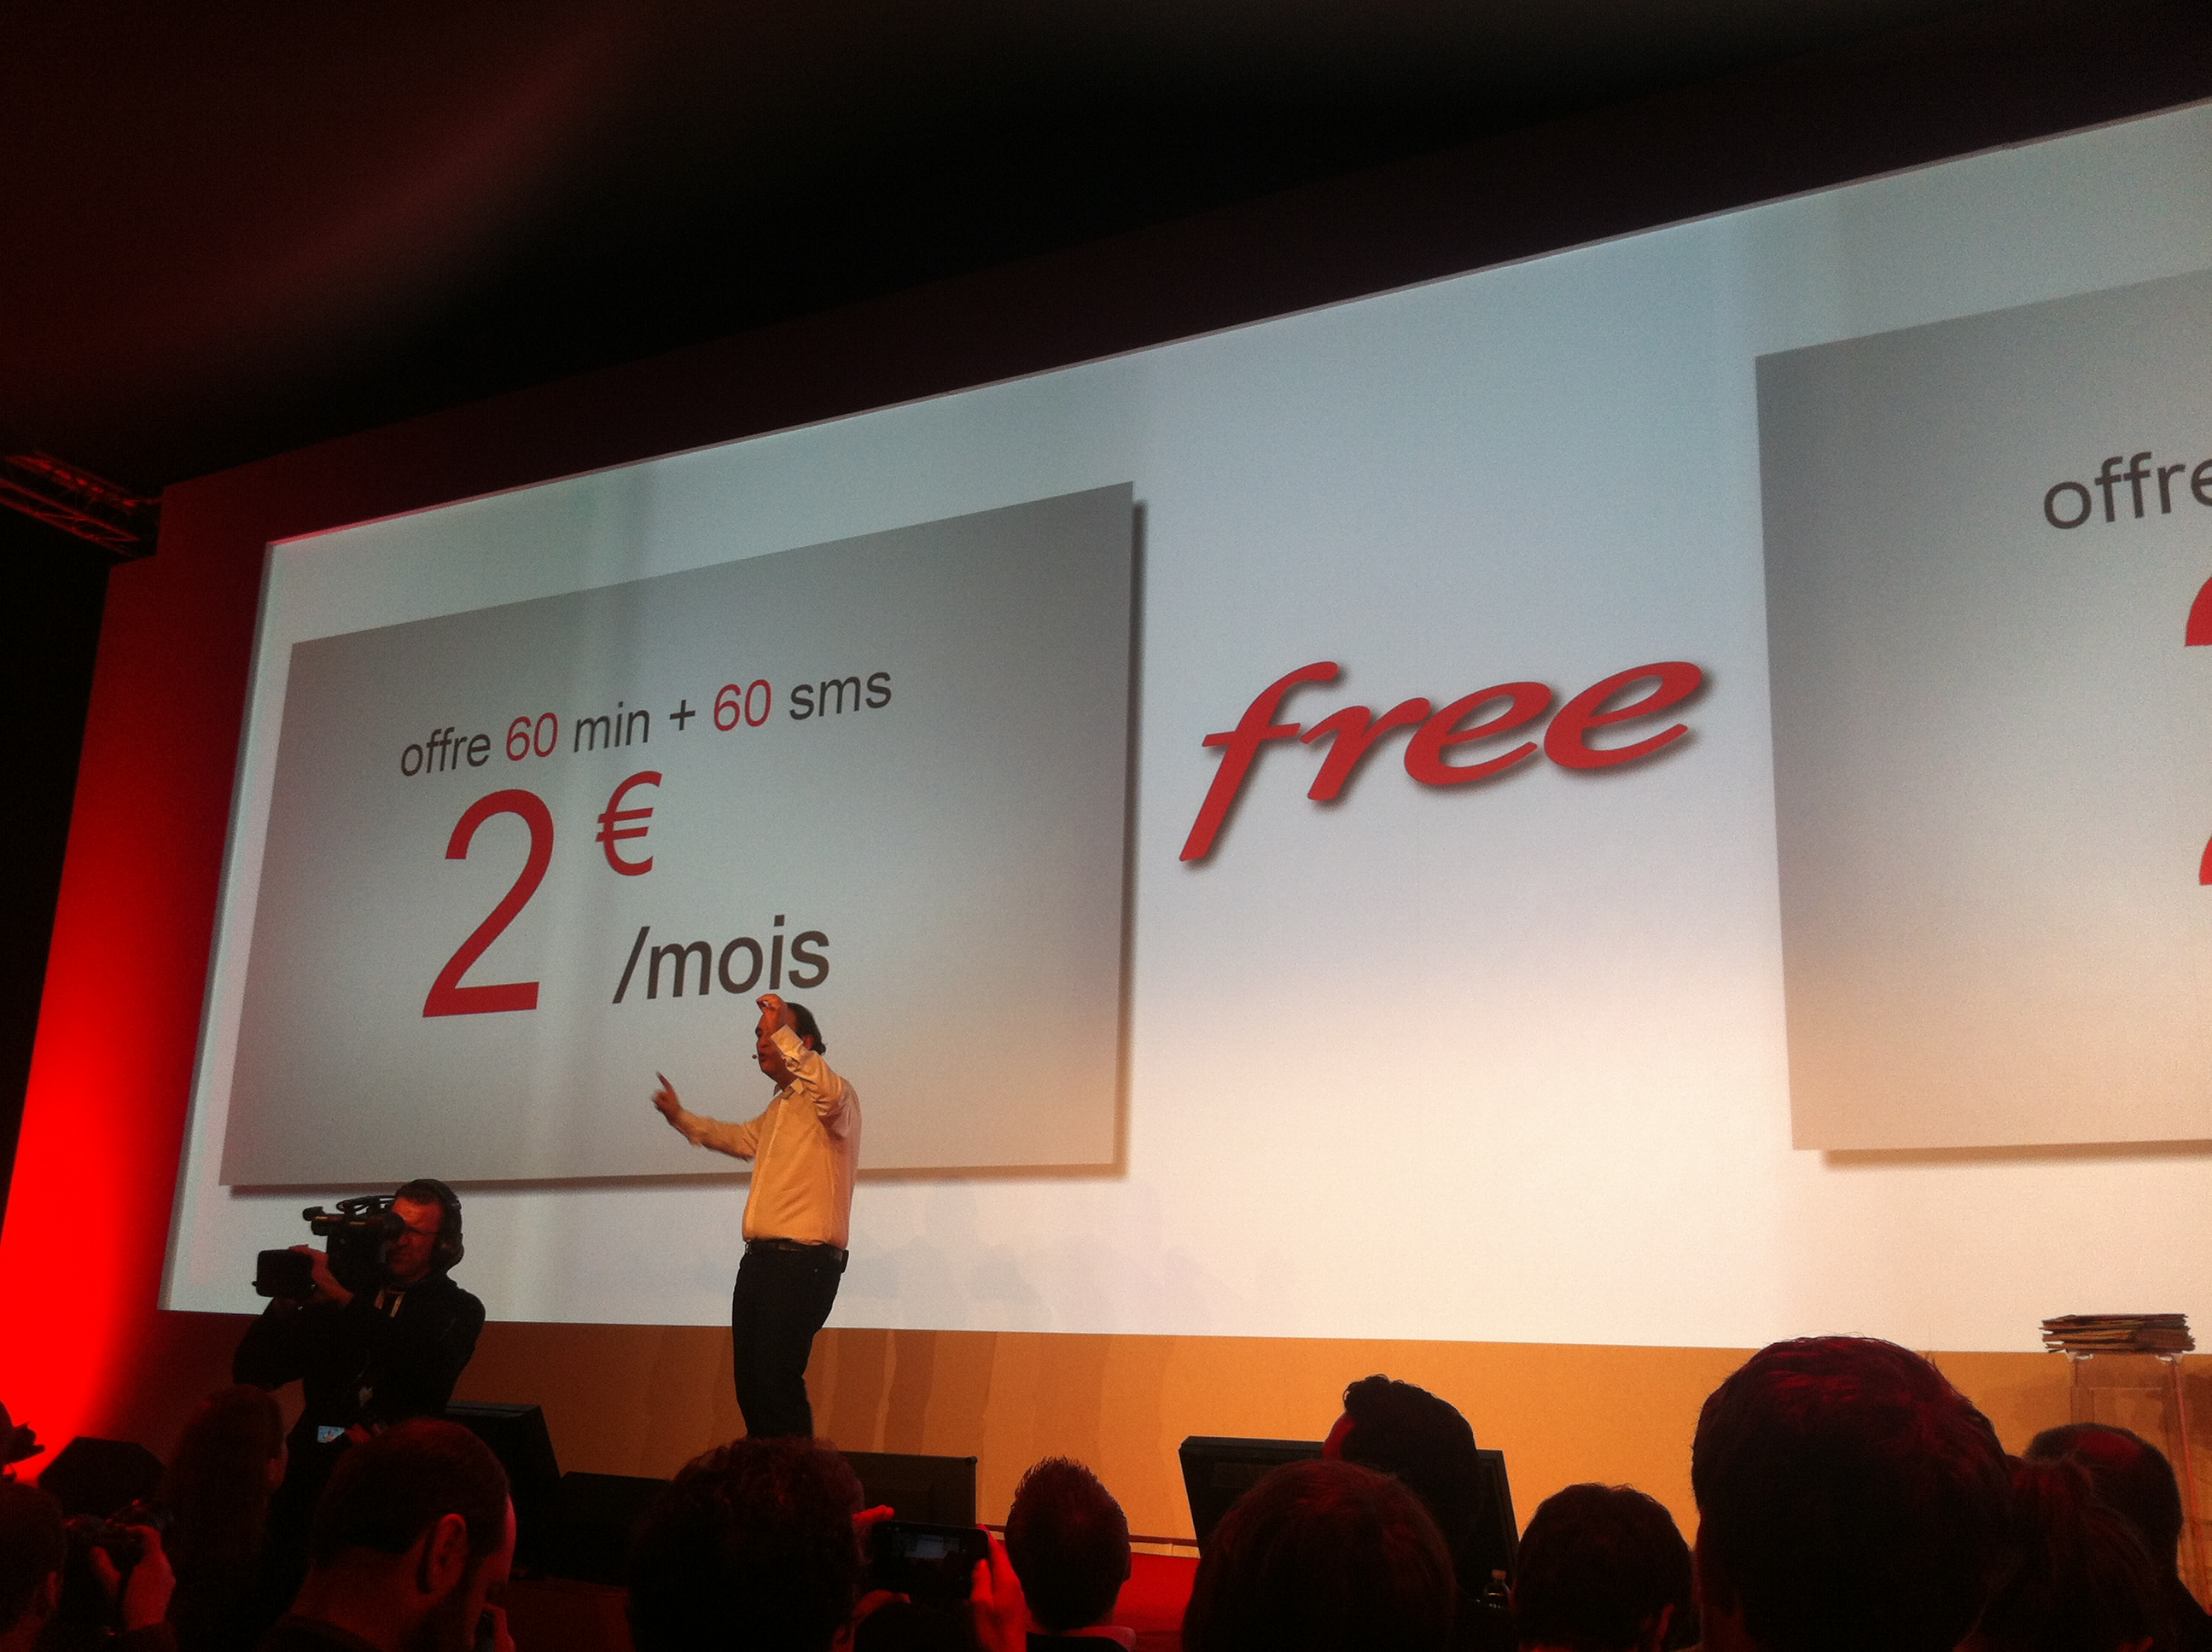
\includegraphics[height=\thumbheight]{resources/free/looseduplicate9.jpg}
		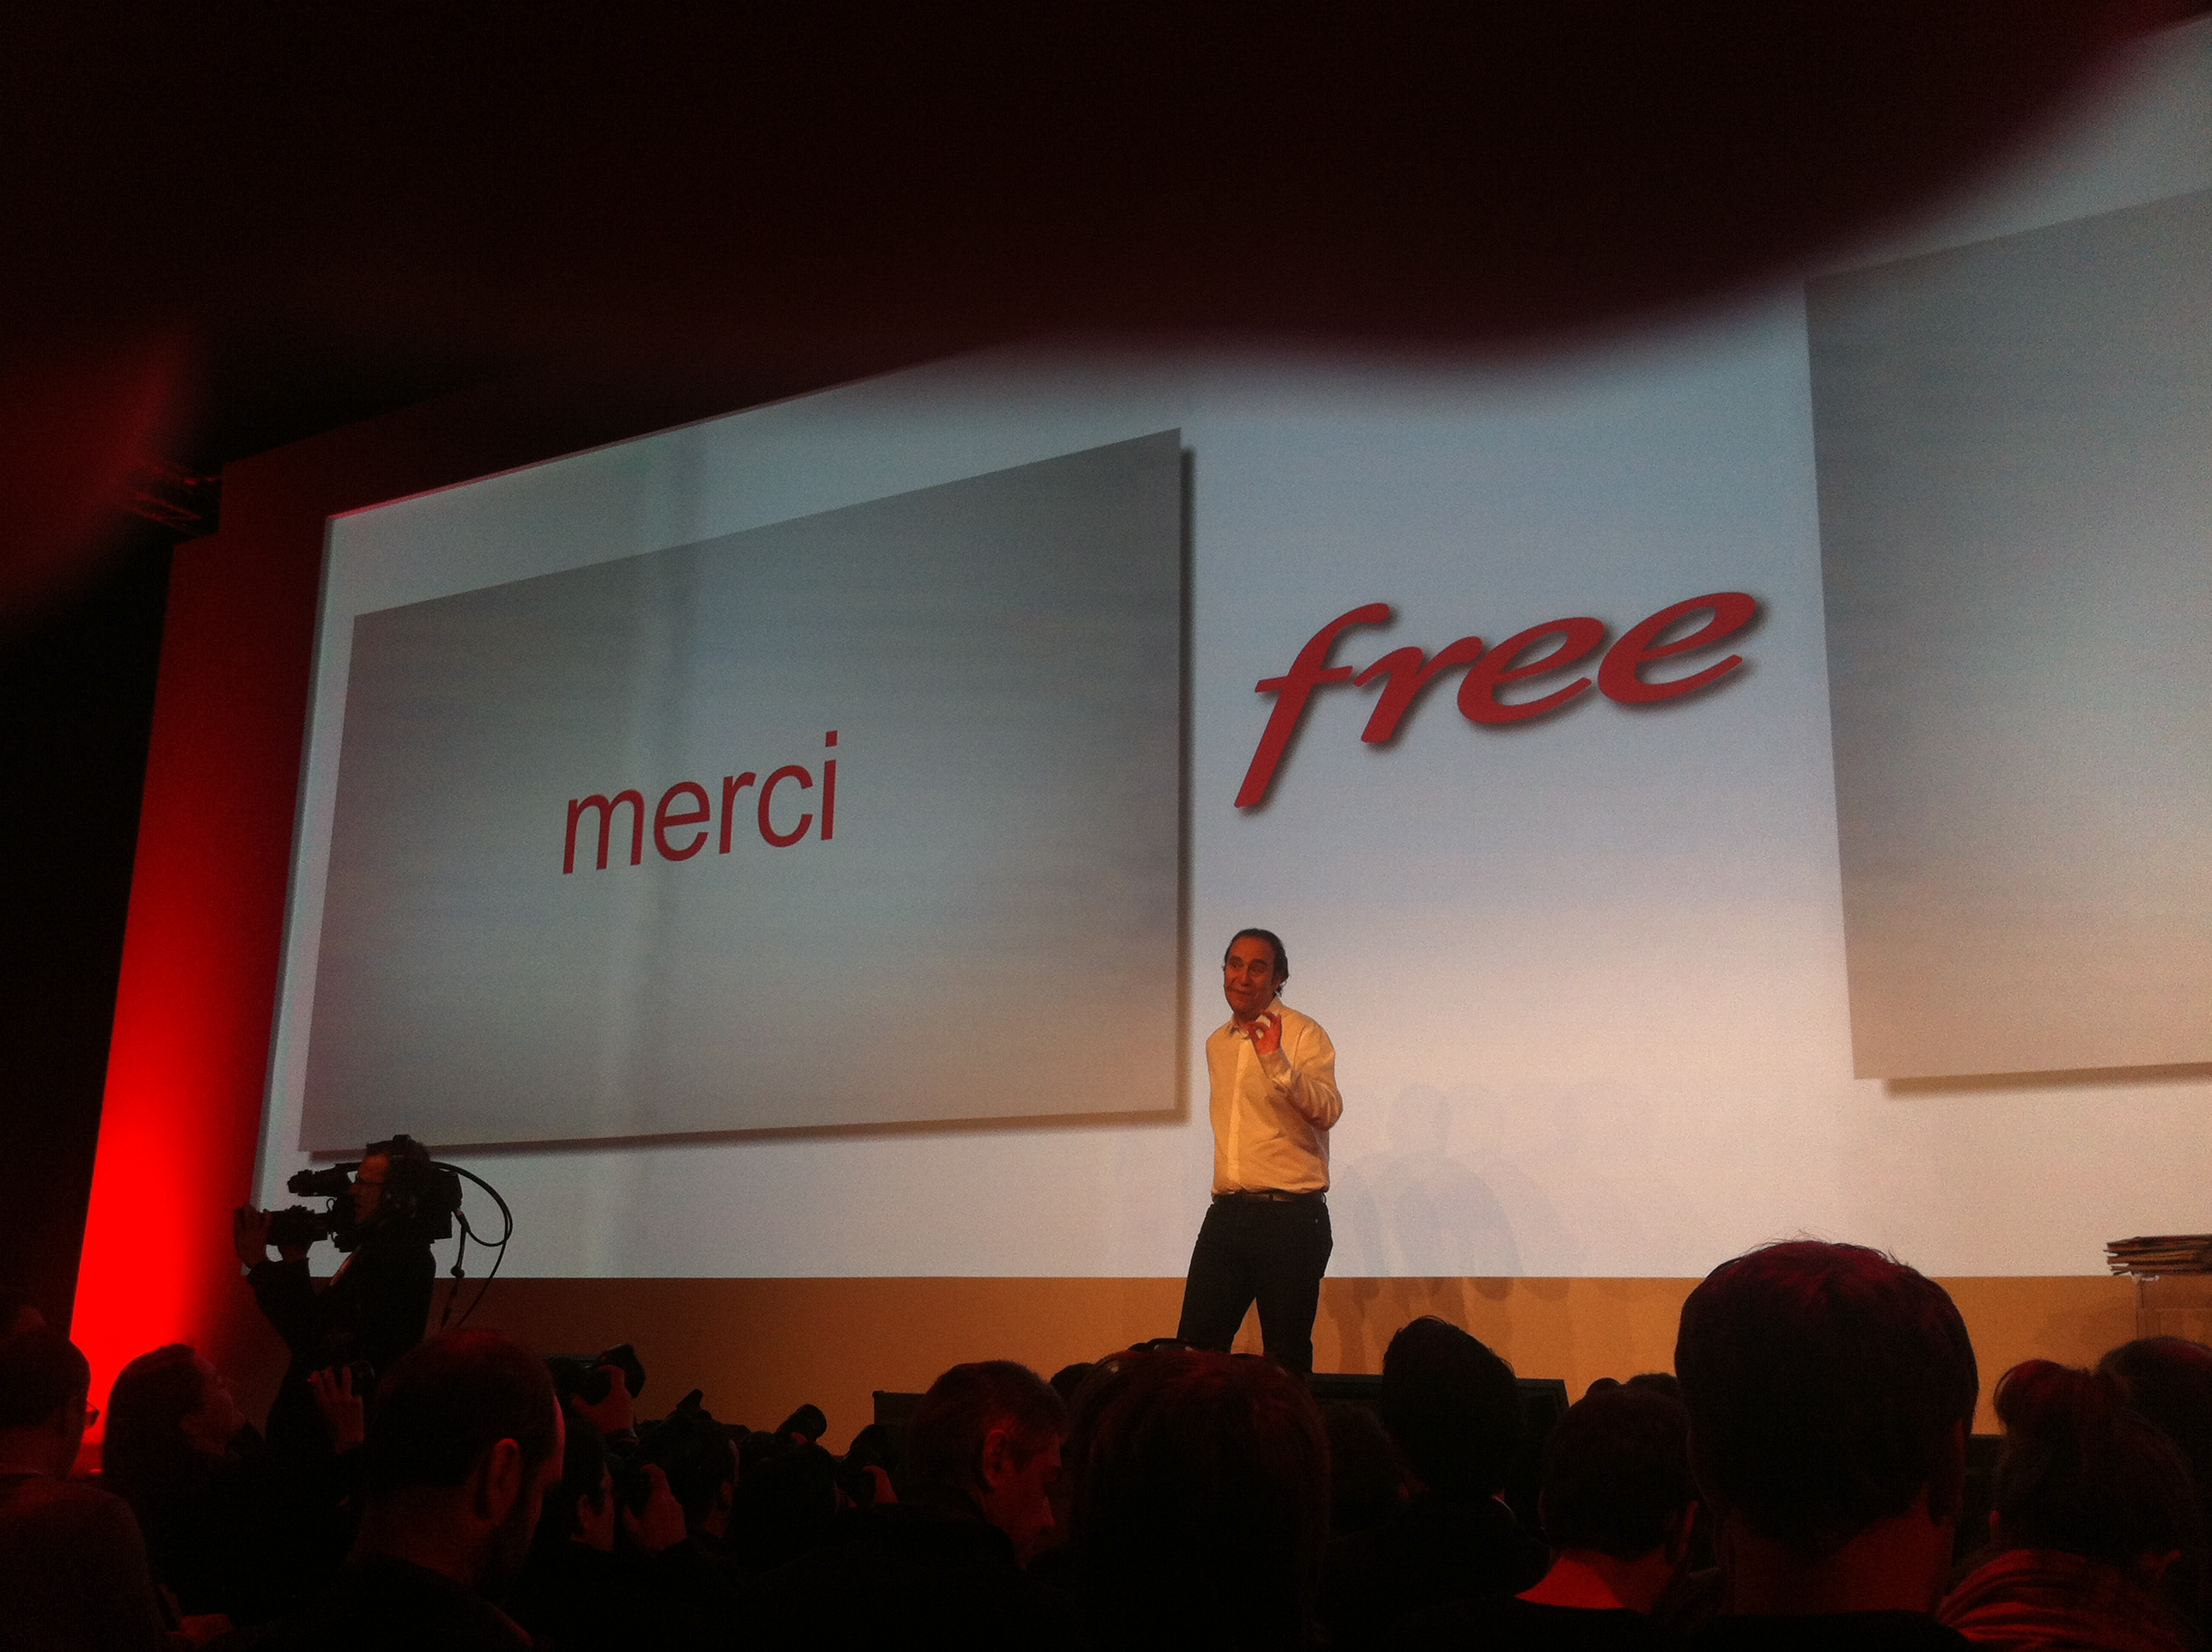
\includegraphics[height=\thumbheight]{resources/free/looseduplicate10.jpg}
		
\includegraphics[height=\thumbheight]{resources/free/looseduplicate11.jpg}
	\end{thumbsequence}
	\begin{thumbsequence}
		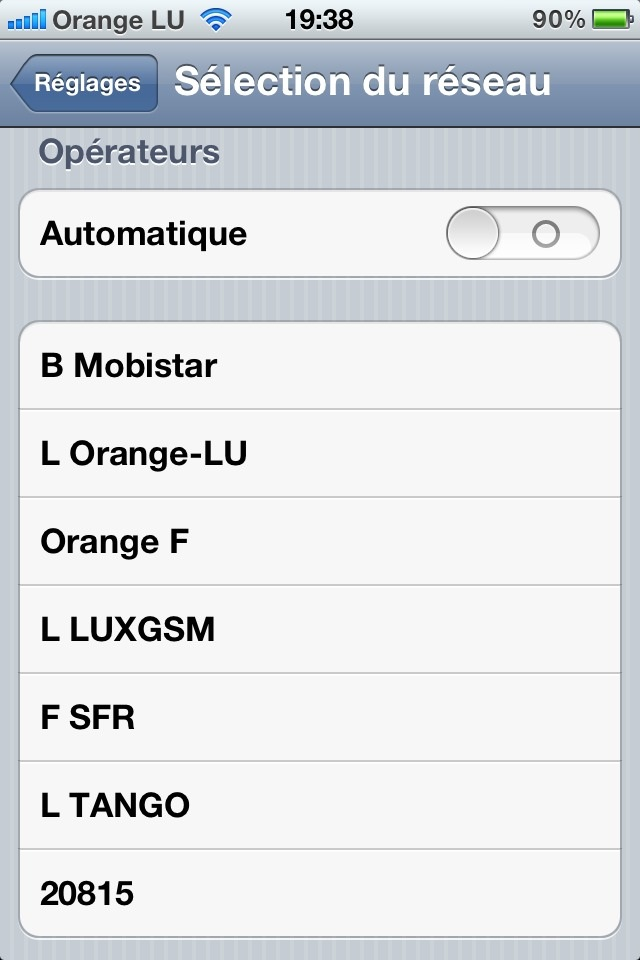
\includegraphics[height=\thumbheight]{resources/free/looseduplicate3.jpg}
		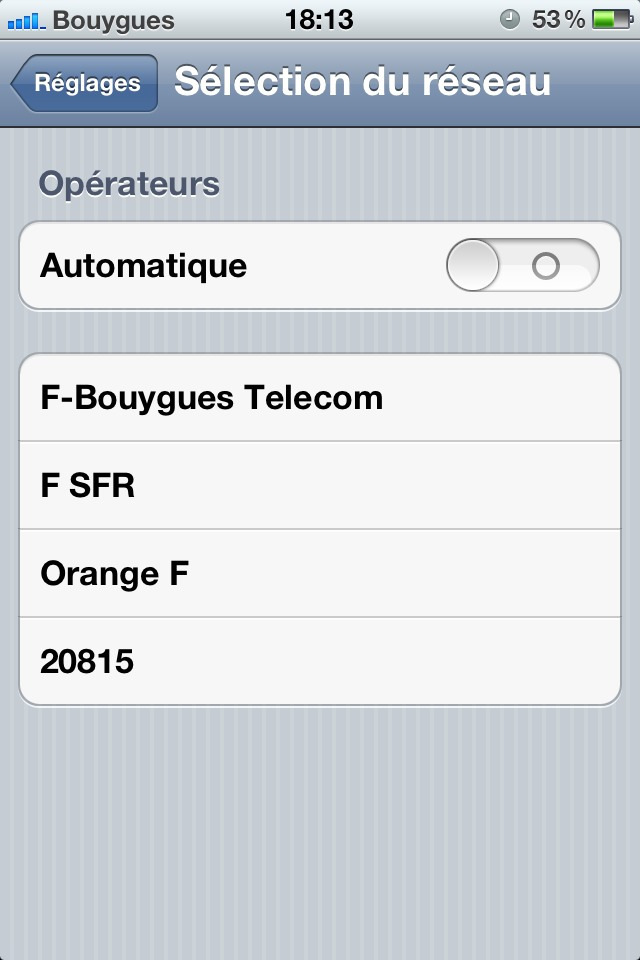
\includegraphics[height=\thumbheight]{resources/free/looseduplicate4.jpg}
	\end{thumbsequence}
	\newstrip
	\begin{thumbsequence}
		
\includegraphics[height=\thumbheight]{resources/free/looseduplicate12.jpg}
		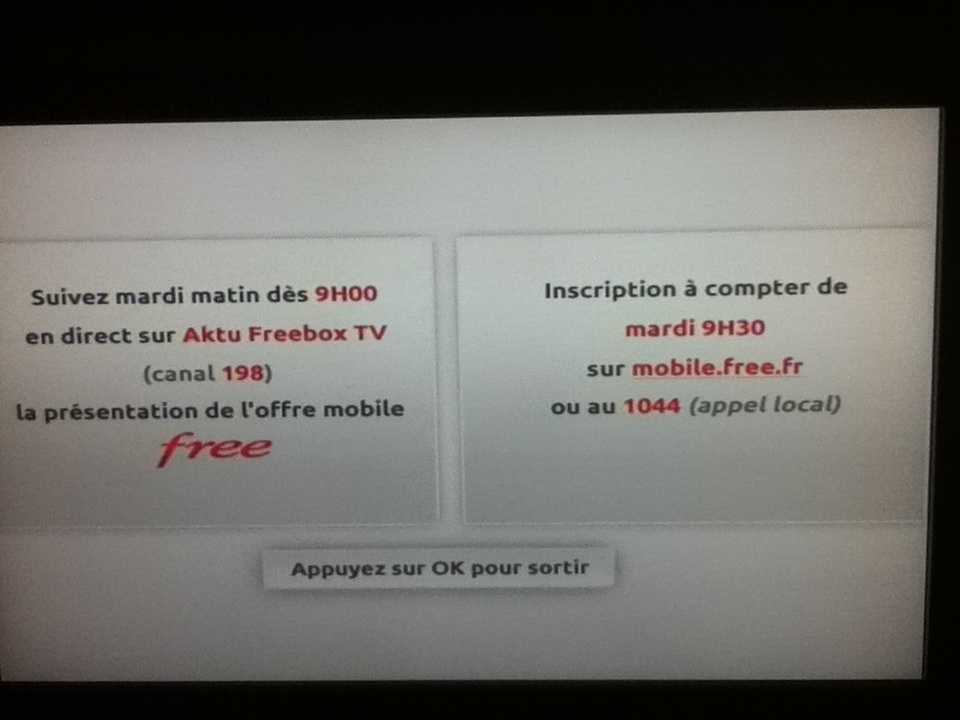
\includegraphics[height=\thumbheight]{resources/free/looseduplicate13.jpg}
		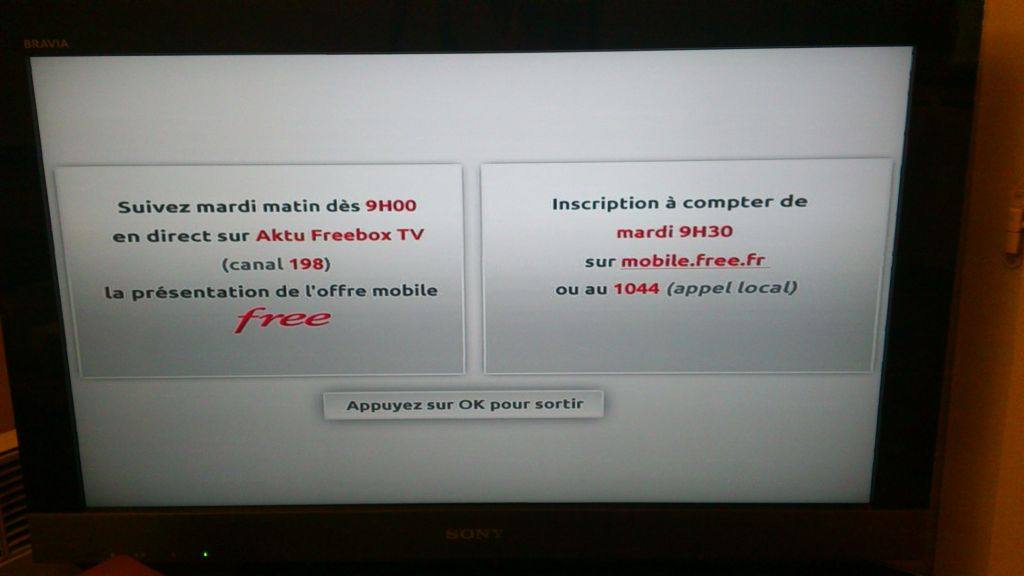
\includegraphics[height=\thumbheight]{resources/free/looseduplicate14.jpg}
	\end{thumbsequence}
	\begin{thumbsequence}
		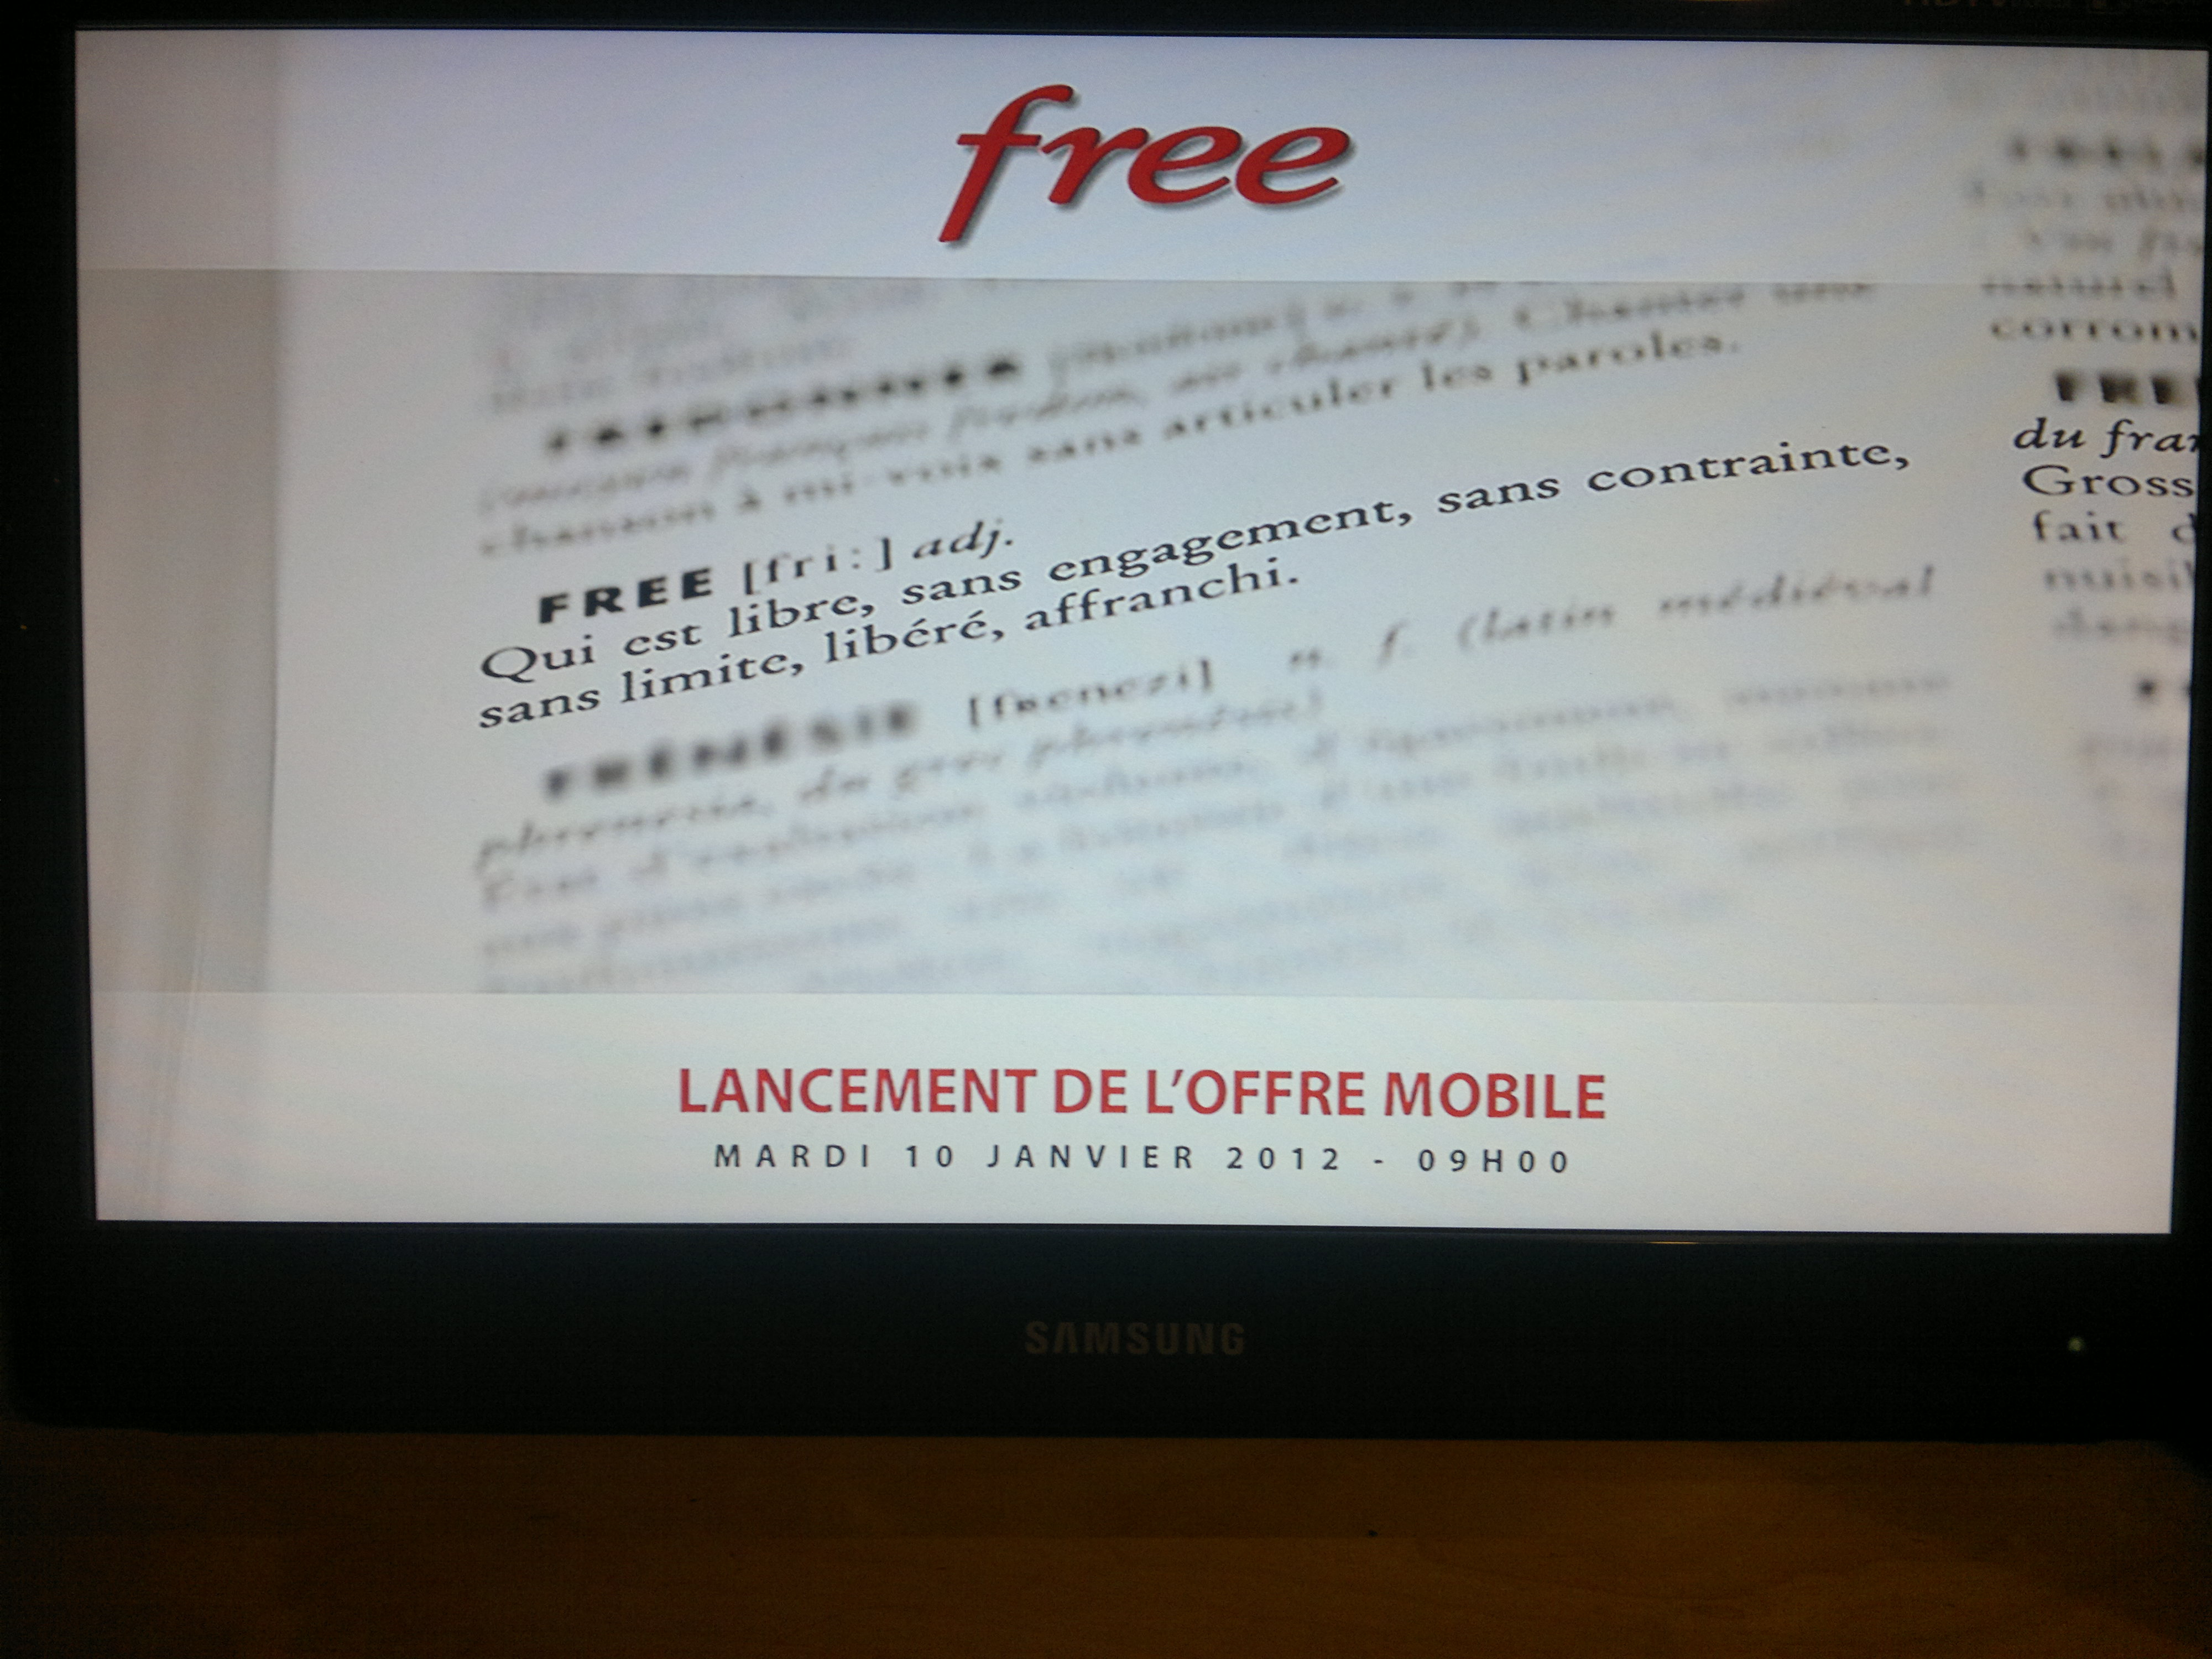
\includegraphics[height=\thumbheight]{resources/free/looseduplicate5.jpg}
		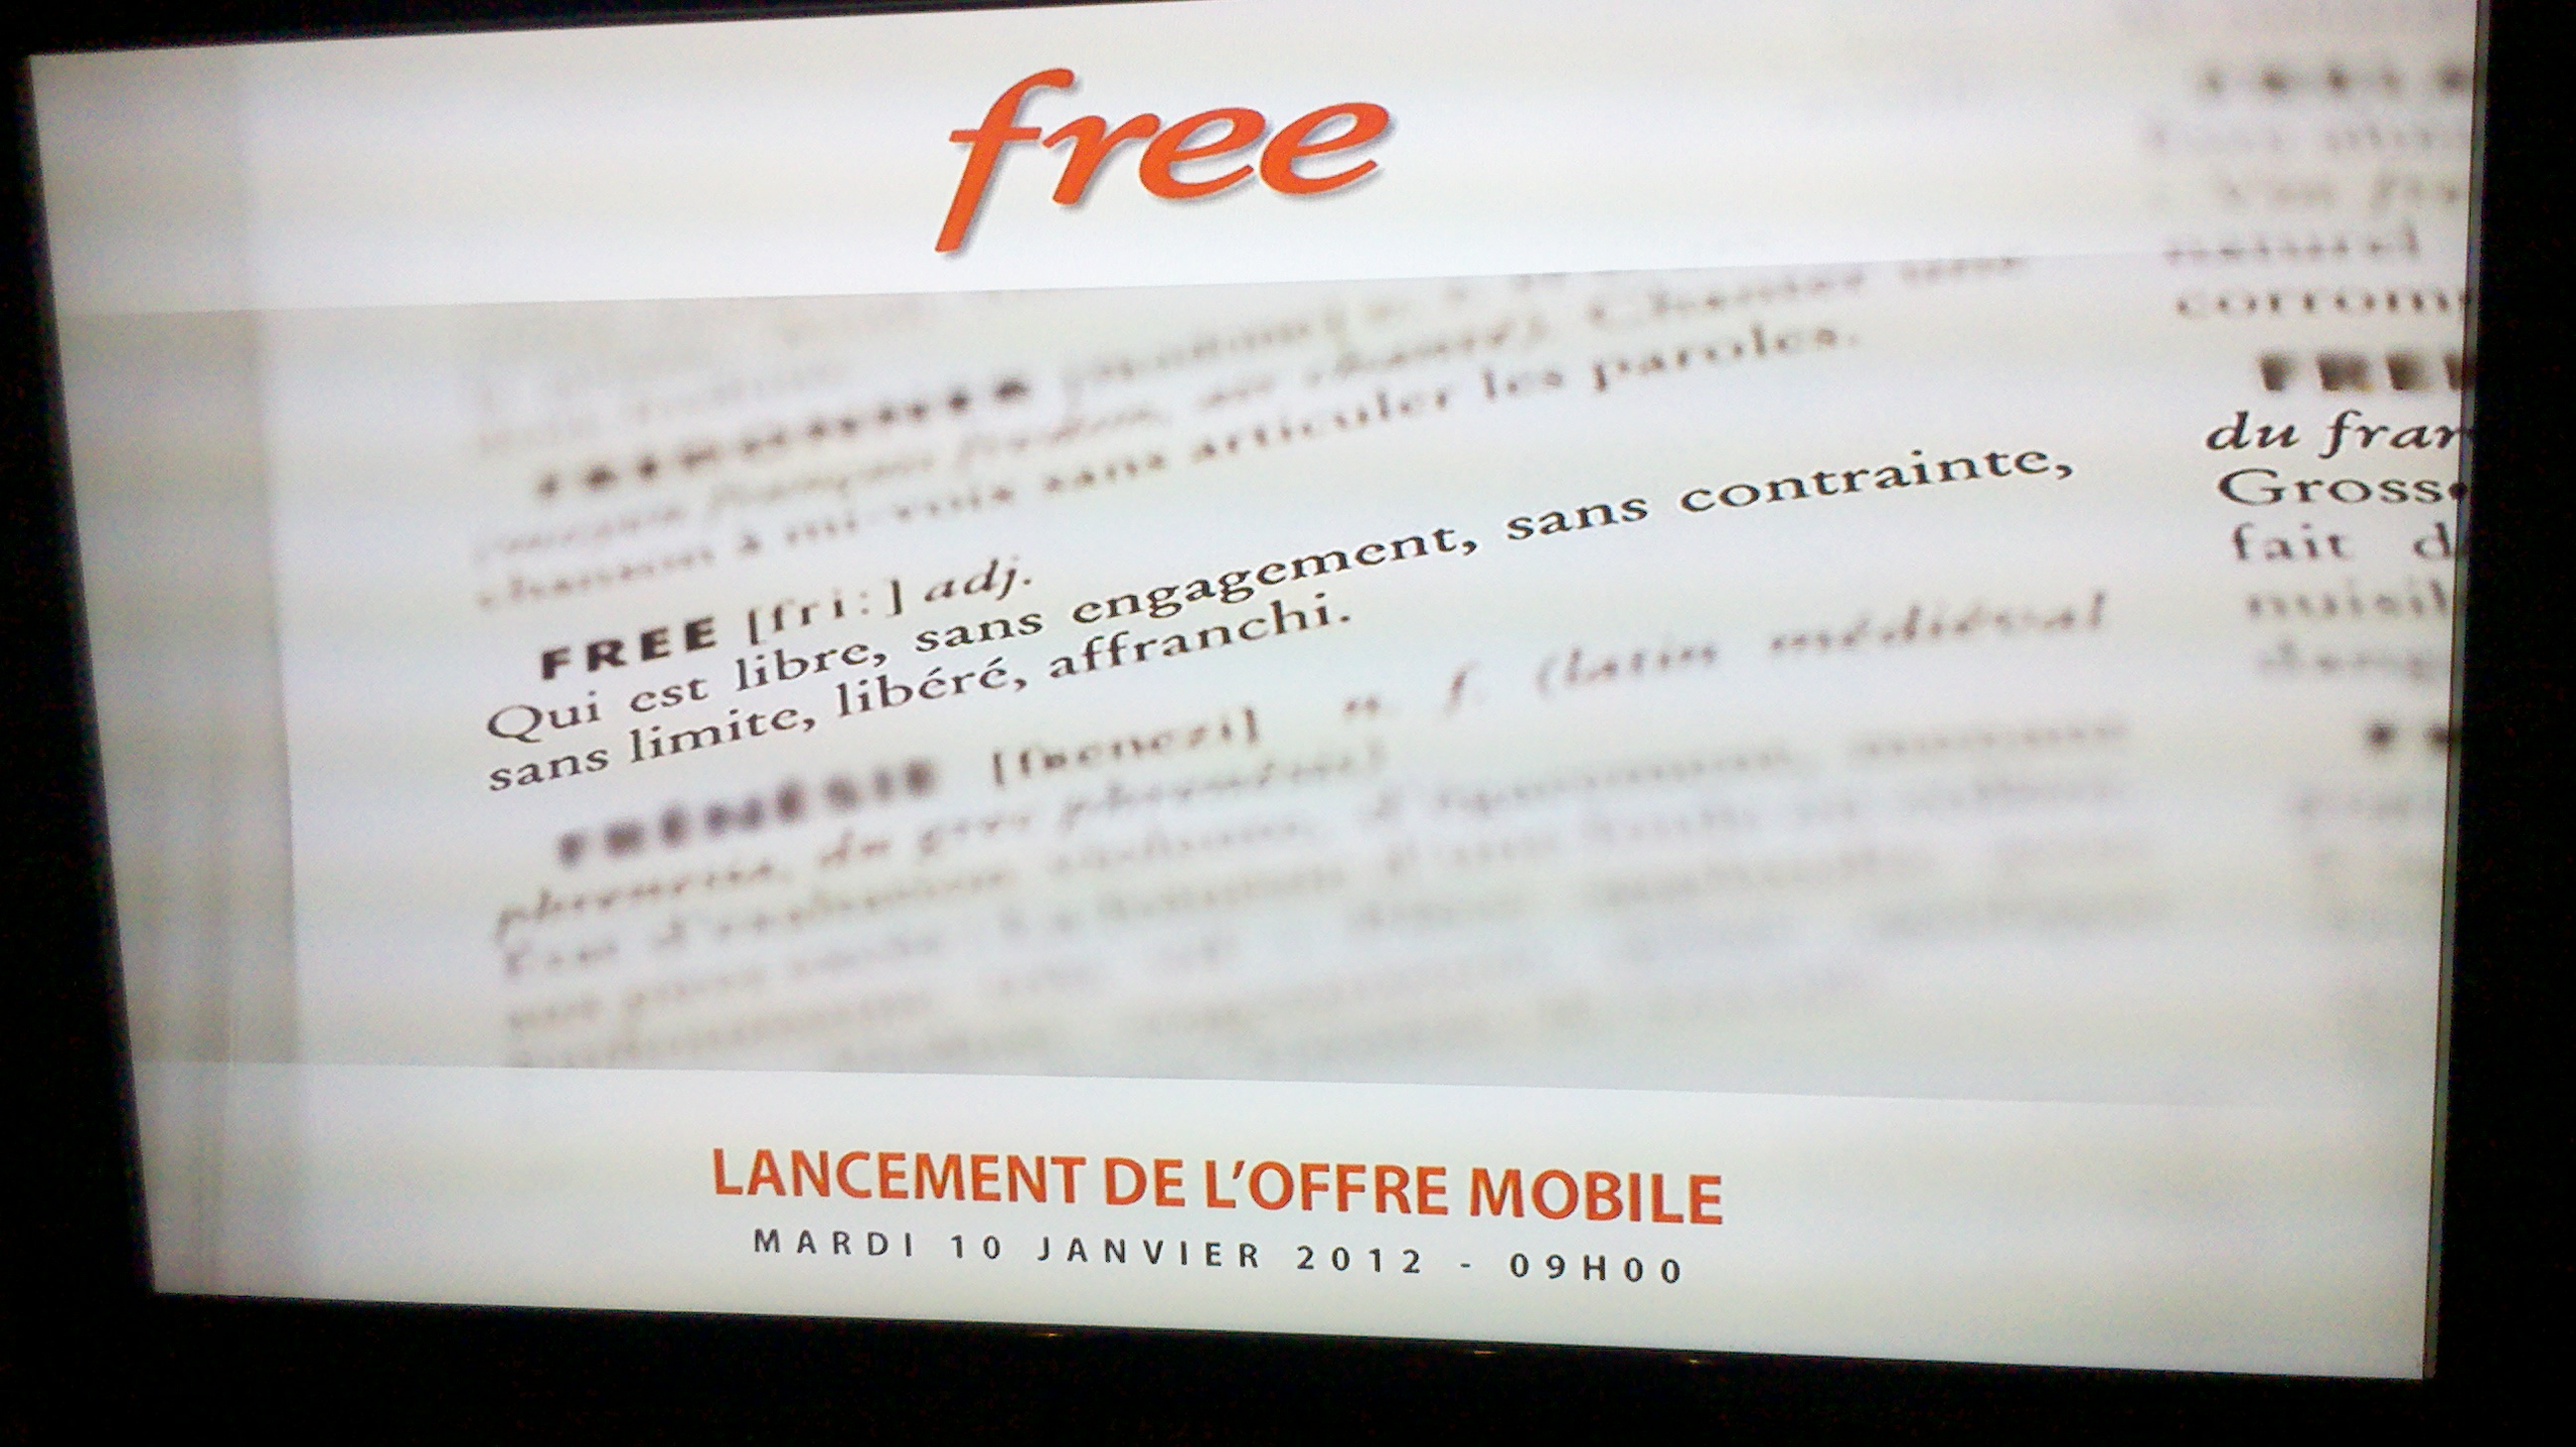
\includegraphics[height=\thumbheight]{resources/free/looseduplicate6.jpg}
	\end{thumbsequence}
\end{tabular}

\vspace{.5em}

\begin{tabular}{p{\textwidth}}
\eventtitle{Costa Concordia Disaster}
	\begin{thumbsequence}
		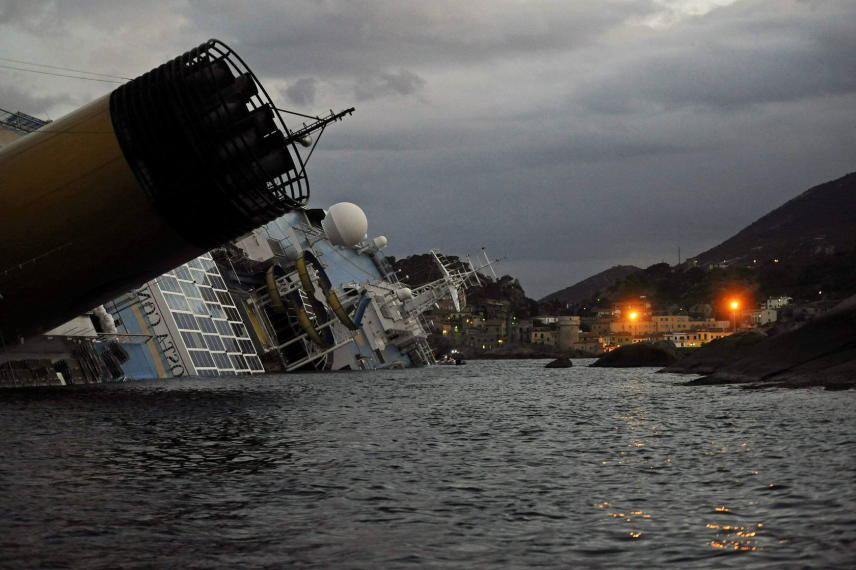
\includegraphics[height=\thumbheight]{resources/concordia/looseduplicate1.jpg}
		
\includegraphics[height=\thumbheight]{resources/concordia/looseduplicate2.jpg}
	\end{thumbsequence}
	\begin{thumbsequence}
		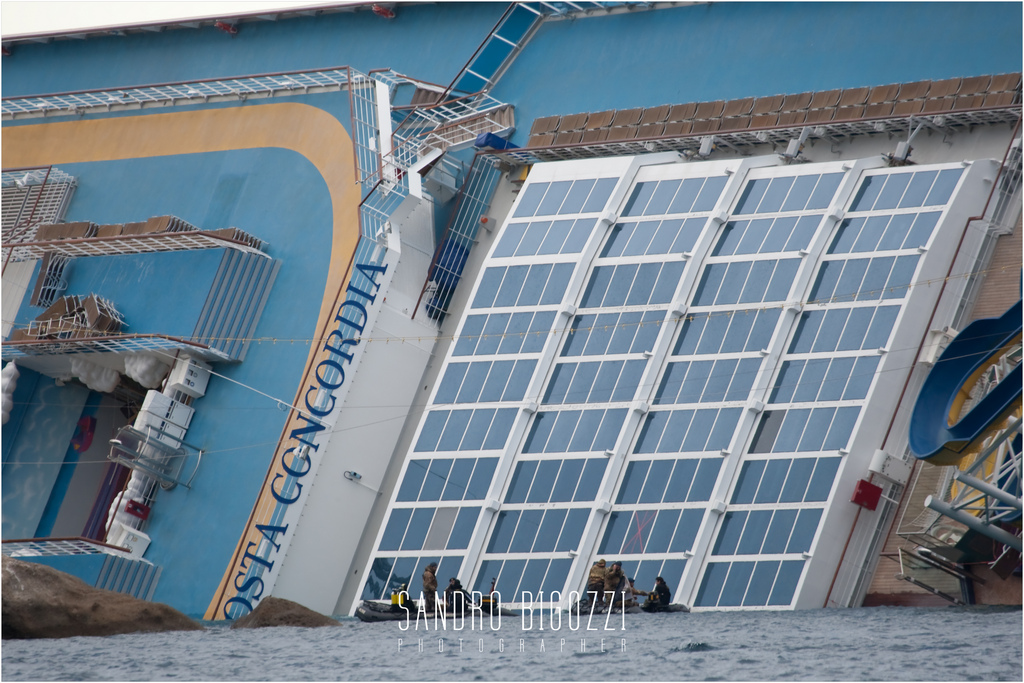
\includegraphics[height=\thumbheight]{resources/concordia/looseduplicate3.jpg}
		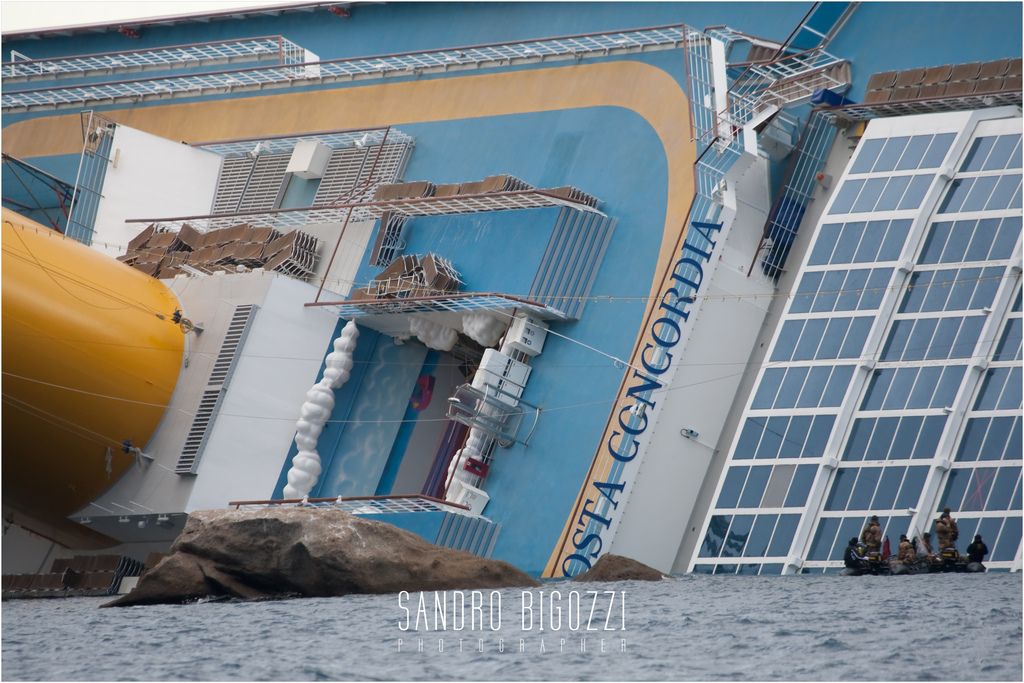
\includegraphics[height=\thumbheight]{resources/concordia/looseduplicate4.jpg}
	\end{thumbsequence}
	\begin{thumbsequence}
		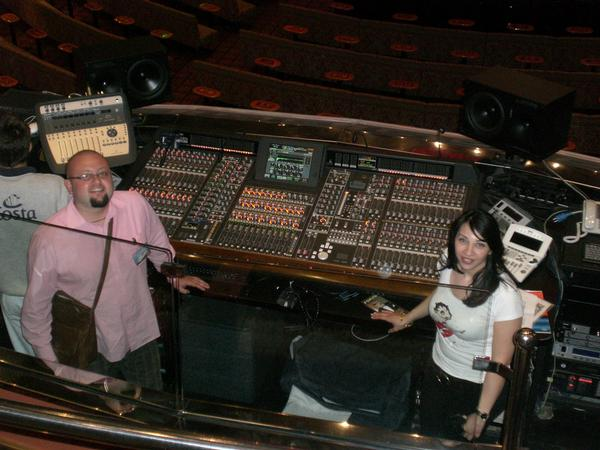
\includegraphics[height=\thumbheight]{resources/concordia/looseduplicate5.jpg}
		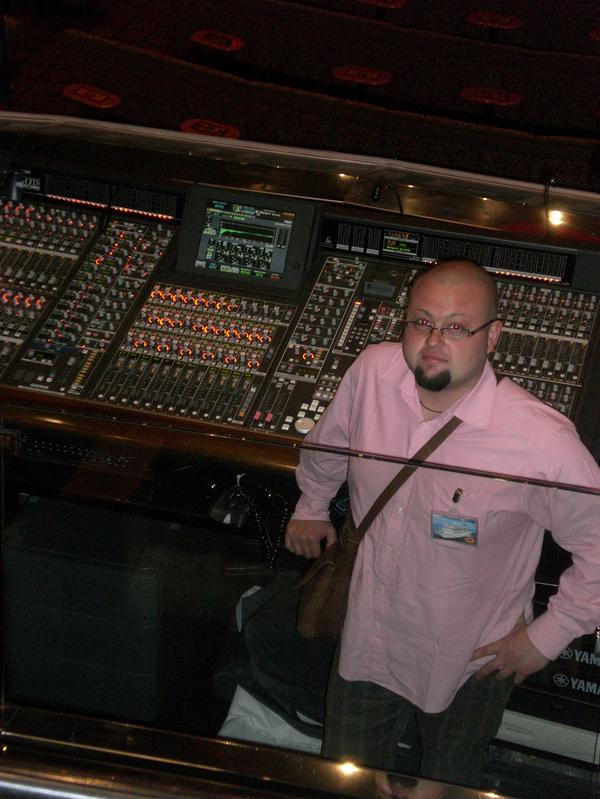
\includegraphics[height=\thumbheight]{resources/concordia/looseduplicate6.jpg}
	\end{thumbsequence}
\end{tabular}

\vspace{.5em}

\begin{tabular}{p{\textwidth}}
\eventtitle{CES Las Vegas}
	\begin{thumbsequence}
		\includegraphics[height=\thumbheight]{resources/ces/looseduplicate1.jpg}
		\includegraphics[height=\thumbheight]{resources/ces/looseduplicate2.jpg}
		\includegraphics[height=\thumbheight]{resources/ces/looseduplicate3.jpg}
		\includegraphics[height=\thumbheight]{resources/ces/looseduplicate4.jpg}
		\includegraphics[height=\thumbheight]{resources/ces/looseduplicate5.jpg}
	\end{thumbsequence}
	\begin{thumbsequence}
		\includegraphics[height=\thumbheight]{resources/ces/looseduplicate6.jpg}
		\includegraphics[height=\thumbheight]{resources/ces/looseduplicate7.jpg}
	\end{thumbsequence}
	\begin{thumbsequence}
		\includegraphics[height=\thumbheight]{resources/ces/looseduplicate8.jpg}
		\includegraphics[height=\thumbheight]{resources/ces/looseduplicate9.jpg}
	\end{thumbsequence}
\end{tabular}

\vspace{.5em}

\begin{tabular}{p{.5\textwidth}p{.5\textwidth}}
	\eventtitle{Cut the Rope Launch}
	\begin{thumbsequence}
		\doublebox{\includegraphics[height=\thumbheight]{resources/ropes/exactduplicate1.jpg}}
		\doublebox{\includegraphics[height=\thumbheight]{resources/ropes/exactduplicate2.jpg}}
	\end{thumbsequence}
	\begin{thumbsequence}
		\includegraphics[height=\thumbheight]{resources/ropes/looseduplicate5.jpg}
		\includegraphics[height=\thumbheight]{resources/ropes/looseduplicate6.jpg}
		\includegraphics[height=\thumbheight]{resources/ropes/looseduplicate7.jpg}
		\includegraphics[height=\thumbheight]{resources/ropes/looseduplicate8.jpg}
		\includegraphics[height=\thumbheight]{resources/ropes/looseduplicate9.jpg}
	\end{thumbsequence}
	\newline\vspace{-.5em}\newline
	\begin{thumbsequence}
		\includegraphics[height=\thumbheight]{resources/ropes/looseduplicate12.jpg}
		\includegraphics[height=\thumbheight]{resources/ropes/looseduplicate13.jpg}
	\end{thumbsequence}
	\begin{thumbsequence}
		\includegraphics[height=\thumbheight]{resources/ropes/looseduplicate14.jpg}
		\includegraphics[height=\thumbheight]{resources/ropes/looseduplicate15.jpg}
	\end{thumbsequence}
	\begin{thumbsequence}
		\includegraphics[height=\thumbheight]{resources/ropes/looseduplicate10.jpg}
		\includegraphics[height=\thumbheight]{resources/ropes/looseduplicate11.jpg}
	\end{thumbsequence}
	\newstrip
	\begin{thumbsequence}
		\includegraphics[height=\thumbheight]{resources/ropes/looseduplicate1.jpg}
		\includegraphics[height=\thumbheight]{resources/ropes/looseduplicate2.jpg}
		\includegraphics[height=\thumbheight]{resources/ropes/looseduplicate3.png}
		\includegraphics[height=\thumbheight]{resources/ropes/looseduplicate4.png}
	\end{thumbsequence}
	&
\eventtitle{Ubuntu TV launch}
	\begin{thumbsequence}
		\includegraphics[height=\thumbheight]{resources/ubuntu/looseduplicate1.jpg}
		\includegraphics[height=\thumbheight]{resources/ubuntu/looseduplicate2.jpg}
		\newstrip
		\includegraphics[height=\thumbheight]{resources/ubuntu/looseduplicate3.jpg}
		\includegraphics[height=\thumbheight]{resources/ubuntu/looseduplicate4.jpg}
		\newstrip
		\includegraphics[height=\thumbheight]{resources/ubuntu/looseduplicate5.png}
	\end{thumbsequence}
\end{tabular}
\caption{\todo{caption}}
\label{fig:sequences}
\end{figure*}

\subsection{Results Interpretation and Discussion}
Looking at our dataset, it becomes evident that the amount of exact duplicate images and videos is inferior compared to the amount of loose duplicates.
On the one hand, this is owed to applied search operators that exclude reshared microposts like, e.g., ReTweets of the same tweet.
So in order for the same media item to appear twice in our results, two users have to author different microposts referencing the same media item\footnote{Using the same, or a different URL.} rather than just one user resharing a micropost from the other.
On the other hand, it is also owed to our strict definition of exact duplicate, which counts resized versions of the same media item as different.
We argue that this, while at the first sight counterintuitive,
makes sense as someone had to actively process the media item.
A good example is the Blackout SOPA event where the text in the first sequence in \autoref{fig:sequences} is identical, however,
the images have different file sizes, resolutions, and paddings.
This implies that someone has taken the initial image, processed it by, e.g.,
cropping it, and only then used the modified version.
A similar example is the second sequence in \autoref{fig:sequences} of the Costa Concordia Disaster, where the chimney got cut off.

In order to access extracted media items in the future,
it may not be necessary to just store their references.
Users can at any time terminate their accounts on social networks,
delete media items, or change their privacy settings.
In addition to that, social networks themselves can take media items down on government order or enforcing own policies.
We experienced no longer accessible media items in the context of the Assad Speech event.
To be on the safe side, only media items where explicitly the media item owner as well as the social network permit storage by third parties should be stored.
We did, at this point, not consider legal requirements, however,
do note that for potential future exploitation this is indispensable.

By clustering loose duplicate media items in sequences,
we aim at boosting diversity in the returned set of media items for a given event:
if there are many media items for an event,
in the longterm we try to only show the most relevant ones from each sequence.
This will require a media item ranking formula that will include a combination of different categories of ranking criteria:

\paragraph{Visual Features}
Extracted visual features from media items can help judge their quality.
Sharp is better than blurry, higher contrast is better than lower contrast, etc.
An interesting observation can be made with videos: videos with less or just one camera shot are more probable to be produced by amateurs (in tendency more authentic),
whereas videos with more shots are more probable to be produced by professionals (in tendency more official and credible).
Depending on the event, the one might be preferred over the other.

\paragraph{Low-level Features}
Common low-level features like resolution, file size, but also the presence of Exif data for, e.g.,
geolocation, are good quality indicators.
Longer videos are better than shorter videos, higher resolution is better than lower resolution, etc.

\paragraph{Social Features}
Media items belonging to the same sequence can have different popularity,
both globally across social networks, or on specific social networks.
Combining network-specific signals,
like number of ReTweets on Twitter, Likes on Facebook, +1s on Google+, views on YouTube;
and generic signals, like number of comments to a micropost,
a good social popularity indicator can be generated.
This can also include user diversity, i.e.,
featuring content from different users rather than just content from one user.

\paragraph{Textual Features}
Important context is available in form of microposts that accompany media items.
Named entity disambiguation can reveal valuable insights and, in combination with advanced techniques like face recognition,
help make the right media item choices.
If a user sends a micropost containing a media item about a concert, and if via named entity disambiguation the singer can be mapped back to a Linked Data concept,
the media item can be searched for potentially known objects, e.g., the singer's face.
Applying this combination of visual and textual features,
highly relevant media items can be selected.

\subsection{Result Representation}
Given that a media item ranking was available,
the question of result representation raises.
Should more popular media items be displayed bigger, longer, or with a special decoration like a thicker border in comparison to less popular media items?
For videos, the audio part poses a challenge.
In our experiments we have made the interesting finding that intermixing the audio of all videos of an event oftentimes generates a very characteristic ``noise cloud''.
A good example is the Assad Speech event, where a mix of Arabic voices blends nicely with the speech of a US politician.
A different example is the CES Las Vegas event, where the atmosphere of a big exposition with music, announcements, and technical analyses becomes alive.

%%%%%%%%%%%%%%%%%%%%%%%%%
%%%  5. Related Work  %%%
%%%%%%%%%%%%%%%%%%%%%%%%%

\section{Related Work}                                                      \label{sec:related-work}
% Separate related work in fields:
% - media item collection from social networks
% - event summarization

% Highlight what Twitter is doing (most popular image/video)
% Google news top stories
% Automatic gallery creation

A~first category of related work includes research that aims to collect, align, and organize media for trends or events.
Liu \emph{et al.} combine semantic inferencing and visual analysis to automatically find media to illustrate events~\cite{Liu:ICMR11}.
They interlink large datasets of event metadata and media with the Linking Open Data Cloud~\cite{LODcloud}.
Approaches for alignment use visual, temporal, and spacial similarity measures to map multiple photo streams of the same events~\cite{Yang2011}.
Other ways to collect and order media from social networks use user-driven metadata such as geospatial information~\cite{Crandall}.

Another relevant work area is duplicate and near-duplicate media detection.
As evident from several experiments and mentioned in \autoref{subsec:dataset},
providing unique media content to users is still an unsolved problem.
Work on ordinal measures for image correspondence started in the last decade of the 20\superscript{th}~century~\cite{Bhat}.
Recently, Chum \emph{et al.} have proposed a near-duplicate image detection method using MinHash and tf--idf weighting~\cite{Chum}.
A~method for both images and video has been proposed by Yang \emph{et al.}~\cite{Yang}.
Specialized methods for video exist as well~\cite{Min, Wu}, an excellent survey of which has been conducted by Lian \emph{et al.}~\cite{Lian}.

When unique media items have been collected, the remaining task is to summarize events by selecting the most relevant media fragments.
An article by Fabro and B\"osz\"orm\'enyi~\cite{Fabro:MMM12} details the summarization and presentation of events from content retrieved from social media.
Nowadays, many domain-specific methods already exhibit good accuracy, for example in the sports domain~\cite{Li1,Li2}.
However, the challenge in this field is to find methods that are content-agnostic.
Methods that exploit semantic information~(\emph{e.g.}, \cite{Chen}) will likely provide high-quality results in the future,
but today's most relevant summaries are produced by user interaction~\cite{Olsen}.

%%%%%%%%%%%%%%%%%%%%%%%%%%%%%%%%%%%%%%%
%%%  6. Conclusion and Future Work  %%%
%%%%%%%%%%%%%%%%%%%%%%%%%%%%%%%%%%%%%%%

\section{Conclusion and Future Work}                                        \label{sec:conclusion}
\todo{Write conclusion}

% Responsible: Ruben
In this work, the focus has been on extracting visual media and associated textual messages from social networks.
One possibility for future work would therefore be to pursue our efforts in this direction by supporting more social networks and improving our Web scrapers.
This could significantly improve the quantity and diversity of considered media and messages,
given the fact that different kinds of information are shared to different networks.
%~\cite{ConsumersLook}

A~more innovative direction is to incorporate techniques from multimedia analysis into the process,
as this will create a~multi-modal environment where different factors are used to organize social content.
This can start with context-independent analyses, such as the content deduplication techniques discussed in \autoref{sec:relatedwork},
or visual quality metrics~(sharpness, contrast\ldots) to display original and high-quality media more prominent in results.
Furthermore, this identification of original content can allow users to choose a~balance between popularity~(favor omnipresent content) and originality~(promote rare content).

Context-aware multimedia analysis will likely bring a~new range of parameters into play,
since many media items contain a~message that is complementary to the text.
For example, facial detection~\cite{ViolaJones} and eventually recognition~\cite{Wright}
can signify the presence of specific people in a~media fragment.
As visual recognition systems grow more powerful, more objects will eventually be recognizable by machines~\cite{Serre},
which would allow generating \emph{visual hashtags} that describe the content \emph{inside} of the media item.
Extracted features in all three categories~(\emph{textual} -- from the micropost,
\emph{visual} -- from the media item,
and \emph{social} -- from the social network in the form of ReTweets, Likes, +1s\ldots)
can also
serve as ranking criteria, be it in isolation, or in combination by
introducing a~ranking formula.
As a~result, this would also positively influence the diversity of automated summarizations.

Nonetheless, it remains important to view the media and the associated text as a~whole,
since the text could convey a~sentiment about or an~explanation of the visual data.
Using named entity recognition~\cite{NERD,AddingMeaningToMicroposts}, the important semantic elements in the message text can be identified to build an understanding of its meaning.
The contents of the message could subsequently be used to narrow down the search space for visual factors, enabling cross-fertilization between the textual and visual analysis, which results in effective, context-aware analysis possibilities~\cite{verborgh_mtap_2011}.

%%%%%%%%%%%%%%%%%%%%%%%%%
%%%  Acknowledgments  %%%
%%%%%%%%%%%%%%%%%%%%%%%%%

\section*{Acknowledgments}
The research activities as described in this paper were funded by Ghent University, the Interdisciplinary Institute for Broadband Technology (IBBT), the Institute for the Promotion of Innovation by Science and Technology in Flanders (IWT), the Fund for Scientific Research Flanders (FWO Flanders), and the European Union.

This work was partially supported by the European Commission under Grant No. 248296 FP7 \mbox{I-SEARCH} project.
Joaquim Gabarr\'o is partially supported by TIN-2007-66523 (FORMALISM), and SGR 2009-2015 (\mbox{ALBCOM}).

%%%%%%%%%%%%%%%%%%%%%%
%%%  Bibliography  %%%
%%%%%%%%%%%%%%%%%%%%%%

% back to normal size Computer Modern for URLs in bibliography
\let\ttdefault\oldttdefault
\let\url\oldurl

\bibliographystyle{abbrv}
\bibliography{icmr2012}

\balancecolumns
% That's all folks!
\end{document} 